\documentclass[dutch]{style/tudelft-report}

\usepackage{acronym}
\usepackage{wrapfig}
\acrodef{sig}[SIG]{Software Improvement Group}
\acrodef{rx}[Rx]{Reactive Extensions}
\acrodef{tfs}[TFS]{Team Foundation Server}
\acrodef{mvp}[MVP]{Minimum Viable Product}

\acrodef{paas}[PaaS]{Platform as a Service}

\acrodef{KNSB}[KNSB]{Koninklijke Nederlandsche Schaatsenrijders Bond}
%\acrodef{label}[acronym]{written out form}
\usepackage{longtable}
\usepackage{array}
\newcolumntype{R}{>{\raggedleft\arraybackslash}p{5cm}}
\usepackage{subfigure}
\usepackage{float}
\usepackage{xspace}

\input{style/sourcecode}

\begin{document}

\def \mylaps {MyLaps\xspace}

%% Use Roman numerals for the page numbers of the title pages and table of
%% contents.
\frontmatter

\title[Bachelorproject]{Vantage Practice}
\author{H.J.\ Banken \\ P.A.\ van Hesteren \\ H.T.D.\ Visser}
\affiliation{Technische Universiteit Delft}
\coverimage{style/cover.jpg}
\makecover

\input{style/titelpagina}

\chapter*{Voorwoord}
\setheader{Voorwoord}

Dit document is het eindverslag van het bachelorproject ``Trainingsapp voor Baansporten'', van de opleiding Technische Informatica op de TU Delft, uitgevoerd door Herman Banken, Patrick van Hesteren en Hylke Visser.

\bigskip

\noindent We willen graag de volgende personen bedanken:

\medskip

\noindent
Coach (TU Delft): Cor-Paul Bezemer\\
Projectbegeleider (Emando): Johan Stokking

\bigskip

\begin{flushright}
{\makeatletter\itshape
    \@author \\
    Delft, April 2014
\makeatother}
\end{flushright}

\tableofcontents

\chapter*{Samenvatting}
\setheader{Samenvatting}

In baansporten is de laatste jaren een ontwikkeling gaande om tijdregistratie te digitaliseren door het gebruik van transponders en detectie-lussen (in de baan). Door deze ontwikkeling zijn nieuwe mogelijkheden ontstaan om ook naast het wedstrijdmoment de sportprestaties in te zien.

Het huidige gebruik van transponders - buiten wedstrijden - is voornamelijk achteraf, terwijl juist tijdens de training zowel sporter als coach het meeste bezig zijn met de prestaties. Het is daarom wenselijk om de resultaten in real-time door te geven aan coaches en sporters zelf. De bestaande oplossingen bieden slechts beperkt inzicht in trainingen, hetgeen de aanleiding voor dit Bachelor Eind Project is geweest.\\

\noindent 
Gedurende dit project is met hulp van de agile ontwikkelmethode SCRUM in combinatie met Team Foundation Server gewerkt aan een applicatie die op een overzichtelijke manier inzicht geeft in trainingen van eigen, maar ook andere sporters. Daarnaast bevat de applicatie een sociale component, waarmee sporters gemotiveerd worden om te blijven/gaan sporten.

Gebruikers kunnen een transponder toekennen aan hun account en groepen aan te maken en/of hier deel in te nemen. Deze groepen bieden hen de mogelijkheid om naast hun eigen resultaten ook andermans resultaten in te zien. Bijvoorbeeld een coach en zijn pupillen. Tevens kunnen zij zich abonneren op andere sporters, handig voor het thuisfront.

Daarnaast bevat dit sociale component ook de mogelijkheid om leaderboards, een soort ranglijst, per verschillende context in te zien. Zo heeft iedere gebruiker zijn eigen records, maar heeft hij ook een positie op de ranglijst van de banen waarop hij gesport heeft en in de groepen waarvan hij deel uitmaakt.\\

\noindent
Om sporters reeds tijdens hun training inzicht te geven in hun prestaties dient alle verkregen data realtime verwerkt en verstuurd te worden naar de mobiele telefoons. Om dit mogelijk te maken draait er in de Microsoft Azure Cloud een server die transponder-doorkomsten verwerkt. De doorkomsten komen binnen vanuit MyLaps, de transponder- en detectielussenleverancier. Vervolgens groeperen we doorkomsten op trainingssessies en ronden, en onderscheiden we de rustperiodes. Het verwerkingsproces steekt vernuftig in elkaar: de beschikbare data wordt steeds een beetje meer verrijkt en steeds naar de applicaties verstuurd.

De applicatie is ontwikkeld met behulp van cross-platform ontwikkel-technieken, waardoor deze relatief eenvoudig uit te brengen is op andere mobiele platformen. De back-end van de applicatie is sport-agnostisch, waardoor deze breed inzetbaar is voor allerlei verschillende soorten baansporten. \\

\noindent 
Uit de enquêtes, die gedurende het project afgenomen zijn onder de doelgroep van de applicatie, is gebleken dat er veel vraag naar een dergelijke applicatie is en de applicatie veel potentie heeft. Ook is er tijdens meetings tussen Emando, de opdrachtgever, en de \ac{KNSB} naar voren gekomen dat de \ac{KNSB} veel interesse heeft in de applicatie en de doorontwikkeling ervan.

Momenteel is de iPhone applicatie klaar om de markt op te gaan, maar uit de enquêtes en vanuit de \ac{KNSB} is naar voren gekomen dat er nog veel functionaliteit is die toegevoegd zou kunnen worden aan de applicatie. Onze aanbeveling is dan ook om de applicatie verder te ontwikkelen en de doelgroep te vergroten door de applicatie ook uit te brengen voor andere platformen.



%% Use Arabic numerals for the page numbers of the chapters.
\mainmatter

\chapter{Inleiding} \label{ch:inleiding} \input{partials/inleiding}

\section*{Opbouw Verslag}

In dit verslag zal allereerst in hoofdstuk~\ref{ch:opdracht-en-omschrijving} de opdracht en het domein van de opdracht worden toegelicht. Vervolgens zal in hoofdstuk~\ref{ch:project-methodologie} de methodologie worden behandeld die tijdens het proces is aangehouden. Hierna zal in hoofdstuk~\ref{ch:systeem-ontwerp-en-implementatie} gedetaileerd worden toegelicht op welke manier het systeem is ontworpen, welke implementatiekeuzes er zijn gemaakt en hoe deze keuzes zijn uitgewerkt. In hoofdstuk~\ref{ch:evaluatie} wordt behandeld hoe de applicatie wordt geëvalueerd met behulp van tests en feedback van verschillende betrokken partijen en mogelijke eindgebruikers. Ten slotte zal in hoofdstuk~\ref{ch:discussie} onder andere worden besproken in hoeverre het project een succes is geweest, wat er moet gebeuren om ook een Android applicatie te kunnen maken en welke invloed bepaalde keuzes hebben gehad op het project. Tenslotte zal in de conclusie, in hoofdstuk~\ref{ch:conclusie} worden aangegeven hoe de applicatie is opgeleverd, zal er een visie gegeven worden op de doorontwikkeling van de applicatie en zal worden besproken welke toekomst wij zien voor de applicatie.

\chapter{Opdracht en Omschrijving} \label{ch:opdracht-en-omschrijving} Emando B.V. is een jong bedrijf dat maatwerksoftware maakt. Momenteel ontwikkelt Emando voor de \acf{KNSB} een nieuw licentie-aankoop- en -beheersysteem, een nieuw wedstrijdadministratiesysteem en een nieuwe schaatstijdendatabase. Naar aanleiding van eerder contact met de \ac{KNSB} over toegang tot de schaatstijdendatabase zijn wij in telefonisch contact gekomen met Johan Stokking van Emando. Tijdens het oriënterende gesprek bleek dat zowel wij als Emando er geïnteresseerd in waren dat wij ons Bachelor Eindproject bij Emando zouden uitvoeren, onder begeleiding van de heer Stokking.

\section{Opdrachtsamenvatting}
In de weken voorafgaand aan het Bachelor Eindproject is in samenspraak met Emando de opdrachtomschrijving gemaakt. Bij het brainstormen zijn de minimale eisen en de mogelijke extra functies bedacht:

\begin{quotation}
\itshape
Het ontwerpen en ontwikkelen van een systeem voor het weergeven en analyseren van (live) recreatieve en trainingsdata in de context van baansporten (bijvoorbeeld schaatsen en baanwielrennen). Dit systeem zal realtime gegevens van de baan, maar ook opgeslagen gegevens uit het verleden, inzichtelijk maken voor sporters, coaches en eventuele toeschouwers (volgers). Daarnaast zal er de mogelijkheid zijn om een sociale component en een competitie element toe te voegen, en een mogelijkheid om aggregatie op data uit te voeren.

Het systeem ondersteunt het sporten: sporters hoeven hun training niet te onderbreken, doordat audio cues en sport-specifieke schermen geïmplementeerd worden. De sociale component bestaat uit het volgen van medesporters c.q. familieleden of vrienden en het delen van resultaten. Het competitie-element zal een virtuele competitie tussen vrienden omvatten.

Technisch gezien zal er een scheiding gemaakt worden tussen de diverse toepassingen (clients) en de API. De API biedt toegang tot realtime data en de diverse modulaire (sport-specifieke) aggregaties, waarbij de mogelijkheid bestaat voor bijvoorbeeld coaches om zich te abonneren op meerdere sporters. De API zal gekoppeld worden op bestaande systemen die data van transponders ontsluiten.
\end{quotation}

Om richting te geven aan het toekomstige applicatie, is de opdrachtomschrijving ambitieus opgesteld. We hebben vanaf het begin de instelling gehad om eerst een minimale versie te maken die werkt, om vervolgens de eerste versie uit te bouwen tot een volwaardige applicatie.

Zoals te lezen is in de opdracht zal er zowel een mobiele applicatie als een back-end systeem ontwikkeld worden. In sectie \ref{sec:programma-van-eisen} worden de elementen uit de opdrachtomschrijving uitgesplitst en omgezet in functionaliteiten met de bijbehorende prioriteit.

\section{Doelgroep en Gebruikers}

\newcommand{\doelgroep}{}
\label{sec:doelgroep}

\subsection*{Schaatsers}
De voornaamste doelgroep van onze applicatie bestaat uit recreatieve en amateurschaatsers. Zij moeten met behulp van onze applicatie meer inzicht krijgen in hun prestaties en trainingen. 
Om ervoor te zorgen dat deze groep gebruikers onze applicatie verkiest boven de reeds bestaande (minder uitgebreide) systemen, dienen zij snel en gemakkelijk met de applicatie aan de slag te kunnen gaan.

Bij een té ingewikkeld systeem zullen zij afhaken en de overstap naar onze applicatie wellicht niet willen maken.
Omdat zij de belangrijkste doelgroep zijn van de applicatie, is het belangrijk dat zij gemotiveerd worden om de applicatie te blijven gebruiken en hen tevens te motiveren om ook anderen aan te sporen dit te doen.
Met behulp van sociale componenten zoals trainingsgroepen, het volgen van andere schaatsers en leaderboards kan onze applicatie hen hierin stimuleren.

\subsection*{Coaches}
De tweede doelgroep bestaat uit de coaches van de schaatsers. Dit zijn mensen die de schaatsers begeleiden bij hun trainingen en wedstrijden. Coaches die zelf niet schaatsen beschikken niet altijd over een transponder, maar zij willen graag snel en gemakkelijk inzicht in de data van de schaatsers die zij coachen. Het moet voor hen dus gemakkelijk zijn om enerzijds snel tussen schaatsers te kunnen switchen en anderzijds de prestaties zowel onderling als per training te vergelijken.

\subsection*{Overige gebruikers}
Tot slot is er de groep gebruikers die zelf geen deel uitmaakt van de schaatswereld. Zij zijn geen schaatsers of coaches en zijn met name geïnteresseerd in de mogelijkheden van de applicatie en het volgen van kennissen of bekende schaatsers.
Ook zij moeten, weliswaar in mindere mate, in staat zijn om de applicatie te gebruiken.

\section{Reeds bestaande vergelijkbare systemen}

\newcommand{\vergelijkbaresystemen}{}
\label{sec:vergelijkbare-systemen}

Er bestaan al enkele oplossingen die functionaliteit bieden die vergelijkbaar is met die van de applicatie die wij gaan bouwen. Strava (Figuur~\ref{fig:strava}) en RunKeeper (Figuur~\ref{fig:runkeeper}) maken gebruik van GPS om onderandere hardlopers en wielrenners van realtime informatie te voorzien. MyLaps Practice (Figuur~\ref{fig:mylapspractice}) is een website waar je na je training je prestaties kan terugkijken. Er bestaat ook een iPhone App voor MyLaps Practice (Figuur~\ref{fig:mylapspractice-app}). Coach Watch (Figuur~\ref{fig:coachwatch}) is een iPad applicatie waarmee coaches hun teams kunnen volgen.

\begin{figure}[ht]
\centering
\subfigure[Strava]{
    \includegraphics[height=5cm]{style/images/Strava}
    \label{fig:strava}
}
\subfigure[RunKeeper]{
    \includegraphics[height=5cm]{style/images/RunKeeper}
    \label{fig:runkeeper}
}
\subfigure[Coach Watch]{
    \includegraphics[height=5cm]{style/images/CoachWatch}
    \label{fig:coachwatch}
}

\subfigure[MyLaps Practice]{
    \includegraphics[height=7cm]{style/images/MyLapsPractice}
    \label{fig:mylapspractice}
}
\subfigure[MyLaps Practice App]{
    \includegraphics[height=7cm]{style/images/MyLapsPractice-App}
    \label{fig:mylapspractice-app}
}

\caption{Soortgelijke oplossingen}
\label{fig:soortgelijke-oplossingen}
\end{figure}

Strava en RunKeeper zijn voor baansporten, zoals bijvoorbeeld schaatsen, niet goed bruikbaar, aangezien GPS op de banen slecht presteert, waardoor de informatie niet nauwkeurig goenoeg is. MyLaps Practice en Coach Watch maken wel gebruik van de detectielussen in de banen. De MyLaps Practice website kan alleen gebruikt worden voor het achteraf bekijken van sportprestaties en de App is vooral gericht op motorsporten. CoachWatch is een (vrij dure) applicatie die vooral gericht is op coaches en dus minder geschikt voor trainingen of amateursporters.

Emando ziet de mogelijkheid om een applicatie te bieden die gebruikmaakt van de detectielussen in de banen, live gegevens kan tonen op een smartphone en ook nog eens goedkoop of gratis is. Onze applicatie richt zich dus op het invullen van de stukken die missen in de bestaande oplossingen.
    
    % systemen in ontwikkeling bij Emando
\section{Programma van eisen} % MoSCoW shizzle

\newcommand{\programmavaneisen}{}
\label{sec:programma-van-eisen}

Traditioneel gezien wordt bij software ontwikkeling het MoSCoW model gebruikt. Het MoSCoW model onderscheid functionaliteiten op basis van prioriteiten. De verschillende niveau's zijn must-, should-, could- en won't-haves. De vertaling van deze niveau's spreekt voor zich.

Wij gebruiken het in combinatie met SCRUM veel gebruikte \acf{mvp} model. Hierbij wordt gedefinieerd wat het product minimaal moet kunnen om bruikbaar te zijn. In die zin komt onze \ac{mvp} dus overeen met de must-haves uit het MoSCoW model. Eventuele tegenslagen mogen er niet toe lijden dat het \ac{mvp} niet gemaakt wordt, daarom is de planning om het \ac{mvp} al in de 4e week af te hebben. Gebruikers kunnen op dat moment met de applicatie spelen en de kern-functionaliteit beoordelen.

Het \ac{mvp} biedt op zich zelf nog niet alle features die zowel wij als de opdrachtgever graag geïmplementeerd zouden willen zien. Het eindproduct zal over enkele bijzondere functies moeten beschikken, de zogenaamde `killer-features' om het product populair te maken. Deze features zijn in die zin dus vergelijkbaar met de should-haves uit het MoSCoW model.

Na het \ac{mvp} en de features die het verschil maken zijn er ook nog een aantal features die niet noodzakelijk zijn en geen groot verschil zouden maken. Deze features zijn te vergelijken met could-haves uit het MoSCoW model. We zullen zeker niet alle could-haves implementeren, en wellicht komen enkele should-features ook niet aan bod. Wellicht volgt uit een user study dat de door ons bedachte could-haves door users erg gewenste features zijn. In overleg met onze begeleiders kunnen we besluiten deze features te implementeren. Bovendien bieden de could-haves een goede leidraad bij toekomstige ontwikkeling na afloop van ons project.

\subsubsection{Must-haves (\ac{mvp})}

\begin{itemize} \parskip0pt \parsep0pt
    \item Bruikbaar als applicatie op smartphone(s)
    \item Architectuur is sport-agnostisch
    \item De sport-specifieke weergave van tijden is voor schaatsbanen geïmplementeerd
    \item Mogelijkheid om een account aan te maken
    \item Real-time transponder doorkomsten tonen van geselecteerde sporters
    \item Historische doorkomsten van een persoon, gegroepeerd per dag of training
    \item De voor bovenstaande features ontwikkelde API, moet het mogelijk maken om de API uit te breiden en de applicatie aan te passen.
\end{itemize}

\subsubsection{Should-haves}

\begin{itemize} \parskip0pt \parsep0pt
    \item Mogelijkheid om account te koppelen aan Facebook
    \begin{itemize}
        \item Mogelijkheid om prestaties en records te delen op Facebook
    \end{itemize}
    \item Audio-cues geven aan sporter over doorkomsten van een geselecteerde transponder
    \item Leaderboards tonen met sporters gerangschikt naar prestaties en disciplines (virtuele competitie), zoals:
    \begin{itemize}
        \item rondetijd (actuele/gemiddelde/snelste)
        \item snelheid (gemiddelde/snelste)
        \item cumulatieve afstand (per seizoen/week/training)
        \item rust/intensief-ratio (hoeveelheid rondjes, ratio)
        \item achievements-punten (verbeter jezelf 10\%, voor 7 uur op de baan, 2 trainingen per week)
    \end{itemize}
    
    \item Groepen-functionaliteit \begin{itemize}
        \item Mogelijkheid om een lege groep te maken
        \item Mogelijkheid om sporters uit te nodigen voor een groep
        \item Mogelijkheid om op uitnodiging in een groep te gaan
        \item Mogelijkheid om uit een groep te gaan
    \end{itemize}

    \item Zowel leaderboards als real-time doorkomst-schermen kunnen worden gefilterd op groep of baan
     
    \item Privacy instellingen bieden aan gebruikers
    \begin{itemize}
        \item Mogelijkheid om een account publiekelijk of anoniem te laten indexeren
        \item Mogelijkheid om eigen data te delen met anderen
    \end{itemize}

\end{itemize}

\subsubsection{Could-haves}

\begin{itemize} \parskip0pt \parsep0pt
    \item Suggesties krijgen om met soortgelijke schaatsers te gaan schaatsen
    \item Training kunnen exporteren naar RunKeeper\footnote{Fitness logboek platform, \url{http://www.runkeeper.com}}
\end{itemize}

\subsubsection{Won't-haves}

Het door Emando ontwikkelde systeem Vantage zal de huidige systemen voor wedstrijduitslagen vervangen. Koppelingen op het huidige systeem zouden dus snel niet meer werken en het nieuwe systeem is niet af tijdens ons project.
\begin{itemize} \parskip0pt \parsep0pt
    \item Wedstrijdloting en uitslagen bekijken
    \item Persoonlijke records tonen
\end{itemize}


\chapter{Projectmethodologie} \label{ch:project-methodologie} \section{Proces aanpak}

\subsection{Stand up meetings}
Om het overzicht binnen het project te waarborgen, zullen er iedere werkdag aan het begin van de dag stand up meetings met alle projectleden plaatsvinden. Bij deze stand up meetings wordt kort besproken waar momenteel aan gewerkt wordt, in hoeverre dit nog op schema ligt en waar de uitdagingen liggen voor de komende dagen. De opdrachtgever zal minstens twee keer per week aanwezig zijn bij deze meetings, hetgeen naar wens vanzelfsprekend vaker kan.

\subsection{Scrum}
In overleg met de opdrachtgever is er gekozen voor een scrum aanpak voor het project. Scrum is een flexibele manier om software te ontwikkelen. Hierbij gaan we werken in een multidisciplinair team waarmee we in korte sprints, met een vaste lengte van 2 weken, werkende software opleveren en geleidelijk stabiele functionaliteit toe voegen. Een scrum aanpak heeft als voordeel dat na iedere sprint er een werkend product af is, waarna de eisen en doelstellingen gemakkelijk bijgesteld kunnen worden. Met scrum kunnen na de gebruikerstest, halverwege het project, de doelstellingen bijgesteld worden aan de hand van de uitkomst van deze test. Door deze agile methode toe te passen sluit het eindproduct altijd zo goed mogelijk aan op de wensen van de opdrachtgever en de end-users.

\subsection{\acl{tfs}}
Emando gebruikt \ac{tfs} voor het versiebeheer van broncode, het bijhouden van het ontwikkelproces, het tracken van issues en het visualiseren van de voortgang in projecten. De gemakkelijke integratie van \ac{tfs} met Visual Studio zorgt ervoor dat issues en backlog items gemakkelijk toegewezen kunnen worden aan developers, waarna zij deze kunnen openen en hiermee aan de slag kunnen binnen hun IDE. De status van deze items kan zowel vanuit de IDE als online aangepast worden en bij het afvinken van items kunnen deze gekoppeld worden aan versie nummers, zodat deze achteraf makkelijk vindbaar zijn.
Ook zorgt de visualisatie van de zogenaamde ‘burndown’ van het project voor een inzichtelijke manier, waarbij de opdrachtgever in een handomslag de voortgang van het project in kan zien. Daarnaast biedt \ac{tfs} inzicht in de tijd die ieder issue en backlog item kost, hetgeen een goede indicatie is voor de scrum sprint.

\section{Project keuzes}

\subsection{Back-end}

De bestaande systemen van Emando draaien voornamelijk in Microsoft Azure als Cloud Service. Azure biedt onder andere ondersteuning voor projecten met .NET, NodeJS en PHP. Aangezien MyLaps voor ons een belangrijke databron is en de MyLaps SDK alleen voor C\#/.NET beschikbaar is, kan er veel werk bespaard worden door ook deze programmeertaal en runtime te gebruiken. Emando heeft daarnaast een laag over de MyLaps SDK heen geschreven waardoor de SDK bruikbaar is met Reactive Extensions. De andere ondersteunde runtimes voor de back-ends die Azure ondersteunt hebben we overwogen, maar door gebrek aan de MyLaps SDK waren dit geen echte opties.

\subsubsection{Real-time}
De communicatie tussen de back-end en de clients moet een real-time zijn. Real-time wil zeggen dat de server een update naar de client kan sturen. In `normaal' web verkeer kan de server niet op elk moment een bericht sturen naar de client. De server kan alleen reageren op een verzoek van de client, omdat de client geen vast IP-adres heeft en er standaard geen poort open staat. Pas wanneer de client een uitgaand verzoek heeft gaat er een poort open.

Een oplossing hiervoor is WebSockets: bij WebSockets blijft de verbinding open en dus de poort en kan de server op elk moment een bericht sturen, als er bijvoorbeeld een schaatser voorbij komt. Een verbinding openhouden kost wel geheugen op de server en de server heeft dus een maximum aantal verbindingen dat hij kan openhouden. Er bestaan verschillende WebSocket frameworks die je het aanmaken en onderhouden van de verbindingen uit handen nemen. Een hiervan is SignalR voor .NET. Emando heeft SignalR succesvol gebruikt tijdens de Olympische Spelen van 2014 om \url{live.schaatsen.nl} te voorzien van live data en heeft dus de vuurdoop doorstaan. Tijdens de rit van Sven Kramer (of wie dan ook) waren er honderd miljoen miljard gelijktijdige verbindingen in SignalR. We hebben er dus vertrouwen in dat SignalR ook voor ons doel geschikt is. TODO!!

[...]
    % Bestaande systemen Emando: servers in Azure.
    % Azure ondersteunt .Net, NodeJS, etc....
    % Keuze voor .Net back-end vanwege MyLaps SDK
    % Verder biedt .Net LINQ en Reactive Extensions
    % Overige afwogen back-enden Meteor, NodeJS, Play-scala
    % SignalR, dat door Emando al gebruikt is tijdens de Olympische Spelen heeft zichzelf bewezen als een stabiele en schaalbare dataverbinding tussen client en server. 
    
\subsection{Client}
Er zijn tegenwoordig diverse manieren om mobiele applicaties te maken, voor diverse platformen (iOS, Android, Windows Phone). Deze verschillende methodes vereisen verschillende programmeertalen en architecturen. Een groot verschil tussen de verschillende methodes is de hoeveelheid code die kan worden hergebruikt tussen verschillende platformen. De uiterste daarvan zijn gebruiken een compleet gescheiden broncode versus een volledig gedeelde broncode. De volgende methodes hebben we overwogen:

\begin{description}
\item[Native applicatie:] Een native applicatie is een applicatie die ontworpen is voor een specifiek platform. Het design van dergelijke applicaties ligt (meestal) in het verlengde van de richtlijnen voor dit platform en het gebruik van platform specifieke handelingen (gestures) wordt gestimuleerd en gehanteerd binnen de applicatie. Vanwege de richtlijnen en het gebruik van deze gestures, zijn dergelijke applicaties zelfverklarend voor eindgebruikers. Een ander voordeel is dat door de native implementatie, de user interface performance van dergelijke applicaties doorgaans erg goed is.

Een nadeel van native applicaties is dat applicatie code vaak in een platform specifieke programmeertaal wordt ontwikkeld en dat er daardoor 3 complete applicaties ontwikkeld moeten worden om de drie grootste platformen te ondersteunen (iOS, Android en Windows Phone). Het ontwikkelen hiervan kost daardoor vaak veel tijd.
    
\item[Web applicatie:]
Een web applicatie is een applicatie die ontworpen is om op alle (mobiele) platformen te draaien. Deze applicatie is benaderbaar via het web (browsers) en heeft als groot voordeel dat deze maar 1x ontwikkeld hoeft te worden. Ook zijn veel ontwikkelaars bekend met de programmeertalen waarmee gewerkt moet worden (HTML, CSS en JavaScript).
    
Er zijn veel verschillende frameworks om mobiele applicaties te maken en daar ligt ook meteen een groot gevaar: elk framework heeft zijn eigen voordelen en wisselen tussen frameworks kan vaak betekenen dat grote delen van de applicatie opnieuw geschreven moeten worden. Ook tijdens ons project zijn diverse frameworks (Meteor, Angular, Backbone, Ember) ter sprake gekomen en voor elk genoemd framework wist er een projectlid voor- en nadelen te noemen.
    
\textbf{Frameworks:} jQuery Mobile~\cite{jq-mobile}, Sencha Touch~\cite{sencha}, Meteor~\cite{meteor}, AngularJS~\cite{angular}, Backbone.js~\cite{backbone}, Ember.js~\cite{ember}, Ionic~\cite{ionic}, React~\cite{React}
    
\item[Native applicatie met WebView:] Een ander belangrijk nadeel van web applicaties is het feit dat deze niet vindbaar zijn in de app stores. Native applicaties met een WebView\footnote{Een WebView is een soort van browser binnen een applicatie, zonder de mogelijkheid zelf een url in te voeren.} zijn applicaties waarin met behulp van een webview een reeds bestaande web applicatie geladen wordt. Hiermee kan met relatief weinig tijd worden meegeleund op het model van de applicatie winkels en is de applicatie in een klap vindbaar op de plek waar gebruikers zoeken naar applicaties.
    
Een nadeel van deze applicaties is hun performance. De applicatie laadt steeds webpagina's in en bij het wegvallen van de verbinding kan de applicatie doorgaans geen of weinig informatie of user interface tonen. Ook kan er doorgaans geen of weinig gebruik gemaakt worden van gestures. In sommige implementaties van deze applicaties wordt een onderscheid gemaakt tussen de offline user interface en de online web app, wat de performance verbetert en het probleem met het wegvallen van de verbinding oplost. De prestaties, vormgeving en gestures zijn echter vele malen minder praktisch ingericht dan bij een native applicatie. Gebruikers verwachten deze eigenschappen echter wel van applicaties die ze downloaden uit de applicatie winkels.
    
\textbf{Frameworks:} PhoneGap/Cordova~\cite{cordova}, Titanium~\cite{titanium}
    
\item[Cross Compiling: ] Cross Compiling is een techniek om broncode om te zetten naar uitvoerbare bestanden voor de verschillende platformen. Hiermee kan vaak de business- en servicelaag van de applicatie gedeeld worden tussen platformen, en sommige `cross-compilers' ondersteunen ook het delen van de presentatielaag. Vaak is dit echter niet wenselijk, omdat juist op de presentatielaag veel verschil gemaakt kan worden tussen platformen, om beter aan te sluiten bij de verwachtingen van de gebruiker. Met cross compiling wordt tijd bespaard op de business- en servicelaag, welke gebruikt kan worden om een presentatielaag te maken voor meerdere platformen. Applicaties die gemaakt zijn door middel van Cross Compilation zijn niet te onderscheiden van native applicaties (gemaakt in de programmeertaal van het platform) want de uitvoerbare bestanden zijn binair vrijwel gelijk.
    
Een nadeel van Cross Compiling is dat het opzetten van de architectuur direct op een juiste manier dient te gebeuren, hetgeen tijd extra tijd kan kosten. Het later aanpassen van de architectuur heeft tot gevolg dat er voor alle platformen een update nodig is voordat het project weer succesvol compileert. Ook moet er in tegenstelling tot een web app nog steeds voor meerdere platformen ontwikkeld worden.
    
\textbf{Frameworks:} Xamarin~\cite{xamarin}, Adobe AIR~\cite{adobeair}
\end{description}
    
Wisselen tussen methodiek betekent het opnieuw ontwikkelen van de applicatie. Omdat onze applicatie niet alleen een proof-of-concept is, maar bedoeld is voor echt gebruik en doorontwikkeling, is het economischer om direct voor de uiteindelijke methodiek te kiezen.
    
Omdat performance en responsetijd een belangrijke rol speelt binnen onze applicatie, ligt het voor de hand om voor een native of gelijkwaardig presterende aanpak te gaan. Een implementatie met WebView biedt niet de performance waar we naar op zoek zijn. 
    
In overleg met de opdrachtgever is besloten de applicatie te ontwikkelen voor \'e\'en platform met een Cross Compiling-implementatie. Het ontwikkelen van deze applicatie (met de gestelde eisen) voor meerdere platform kost dusdanig veel tijd dat dit ten koste zou gaan van het MVP. Door een goede business- en servicelaag op te zetten, is het later mogelijk om de applicatie uit te rollen naar andere platformen, door enkel de platform specifieke views nog te ontwikkelen.

We hebben voor Xamarin boven andere Cross Compiling implementaties gekozen omdat Xamarin werkt met het .NET framework en dit een paar belangrijke voordelen met zich meebrengt:

\begin{itemize}
\item Het platform .NET biedt LINQ en \acf{rx}. Met LINQ en \ac{rx} kunnen eenvoudig streams aan binnenkomende data efficient afgehandeld worden. Aangezien dit een belangrijk onderdeel is van onze applicatie is dit een groot voordeel.
\item Aangezien we onze server zullen inrichten met SignalR is het fijn dat er al een SignalR component bestaat voor Xamarin. Dit maakt de communicatie met de server een `no-brainer'.
\item Emando gebruikt \acf{tfs} en de integratie van Xamarin met Visual Studio en dus \ac{tfs} zal de eventuele latere doorontwikkeling en aansluiting op de bestaande werkwijze ten goede zou komen. 
    % eerder al genoemd ?= Dit omdat TFS binnen de huidige werkomgeving gebruikt wordt voor vele doeleinden, waaronder versie-nummering, burn-down, scrum etc. TODO: netjes verwoorden 
\end{itemize}

\section{Tools}

Visual Studio, Xamarin Studio, etc



\chapter{Systeemontwerp en -implementatie} \label{ch:systeem-ontwerp-en-implementatie} \section{Globale systeem opzet}

Zoals besproken tijdens de meeting van 23 april (Pagina \pageref{sec:meeting-23-apr}), worden applicaties die Emando ontwikkelt opgedeeld in vier lagen. Deze opzet zullen wij ook aanhouden.

\begin{description}
\item[De presentatielaag] zal de platform-specifieke User Interface elementen bevatten.
\item[De servicelaag] is eigenlijk de API die gebouwd zal worden met behulp van SignalR
\item[De businesslaag] is verantwoordelijk voor het ophalen van de gegevens
\item[De datalaag] omvat de verschillende databronnen: MyLaps, ...
\end{description}
  % 4 lagen
  % - presentatie laag
  % - service laag: API
  % - business laag: analyse en aggregatie
  % - data laag
  
\section{Server design en implementatie}


\section{Client design en implementatie}


\section{Grafische user interface}


\section{Testomgeving}



\chapter{Evaluatie} \label{ch:evaluatie} \section{KNSB Meetings}
Voorafgaand aan het project is niets afgestemd met de \ac{KNSB}. Gaandeweg het project is er vanuit Emando contact opgenomen met de \ac{KNSB} om hun interesse voor dit project te peilen. Hiervoor bleek enorm veel animo. De \ac{KNSB} heeft aangegeven dat een doorontwikkeling van de applicatie wenselijk is. Ook hebben zij aangegeven dat een Android applicatie wenselijk is, om de doelgroepte vergroten.

\section{Enquête \& gebruikerstest}
Om er zeker van te zijn dat de applicatie aansluit bij de wensen van de doelgroep van onze applicatie, hebben wij een enquête afgenomen om de verwachtingen van de applicatie te peilen vlak na de tweede sprint van het project. Door in een vroeg stadium de verwachtingen van de applicatie te peilen, was het mogelijk om de applicatie gedurende het project aan te passen op deze verwachtingen waar nodig. 

Vlak voor de oplevering van het project hebben we nog een gebruikerstest afgenomen om te kijken hoe de uiteindelijke applicatie hiervan bij de doelgroep bevalt. Hierbij zijn tevens vooraf en achteraf aan de test enquêtes en vragen gesteld aan de gebruikers, om zo een goed beeld te kunnen vormen van hun bevindingen. De verkregen inzichten kunnen gebruikt worden bij de verdere doorontwikkeling en de toekomst van de applicatie. Het testplan en de resultaten zijn te vinden in de bijlagen, respectievelijk: .
{\par \bigskip \par \color{red} TODO: referenties naar bijlagen \par \bigskip \par }

\section{\acs{sig} feedback}

{\par \bigskip \par \color{red} TODO: SIG code analyse en resultaten toelichten \par \bigskip \par }

De \acf{sig} heeft onze broncode tweemaal geëvalueerd.

\chapter{Discussie} \label{ch:discussie} {\par \bigskip \par \color{red} TODO: Inleiding \par \bigskip \par }

\section{Product}

\subsection{Hoe ``af'' is de applicatie?}
Bij de oplevering van het project staat er een werkende applicatie die sporters op een gemakkelijke en overzichtelijke manier inzicht geeft in hun trainingen, maar ook in die van anderen. Daarnaast bevat de applicatie een sociale component die sporters kan motiveren om tot het uiterste te gaan. Deze sociale component zorgt er voor dat sporters de applicatie willen blijven gebruiken. De applicatie berust op een robuuste en uitbreidbare API welke goed gedocumenteerd is. Het is daarmee relatief eenvoudig om extra functionaliteit toe te voegen.

\subsection{Verbeteringen}
Hoewel de applicatie voldoet aan de door ons gedefiniëerde MVP, zijn er enkele verbeterpunten welke toevoegingen kunnen zijn aan de applicatie. Zo zou het mogelijk kunnen zijn om realtime training informatie door te geven aan sporters met behulp van audio cues. 
Verder zou de geaggregeerde data gecombineerd kunnen worden met trainingstijden om gebruikersprofielen te creëren, welke gebruikt kunnen worden om gebruikers suggesties aan te kunnen bieden om met andere sporters van gelijkwaardig niveau te gaan sporten.
Ook is het mogelijk om het sociale component verder uit te breiden naar een achievement systeem. 

Tot slot zou ook het delen van prestaties en records en het exporteren van deze data naar RunKeeper een enorme toevoeging zijn voor de applicatie.

\subsection{Android}
Momenteel is de applicatie slechts beschikbaar voor één mobiel platform: iOS. Naast iOS is ook Android een groot platform waar veel gebruikers van onze doelgroep mee werken, hetgeen de \ac{KNSB} reeds aan heeft gegeven in een van de meetings met Emando. Om het bereik van de applicatie te vergroten, is het aan te raden om de applicatie ook uit te rollen voor Android. Vanwege de cross-platform ontwikkeling met Xamarin, is het slechts nodig om de platform specifieke views te schrijven voor dit platform. Om deze reden kan dit met relatief weinig tijd.

\subsection{Is de applicatie een toevoeging op de reeds bestaande markt?}
Hoewel er zeker ruimte is voor toevoegingen van en verbeteringen aan de huidige applicatie, bevat de applicatie een tal van functionaliteiten welke trainingen voor sporters op een overzichtelijke manier inzichtelijker kunnen maken. Naast het inzien van eigen data, is het ook mogelijk om andermans data in te zien, hetgeen een toevoeging is voor trainingsgroepen en coaches. 
Hoewel deze twee aspecten an sich niet nieuw zijn, is de eenvoud en combinatie er van in één applicatie dat wel. Verder is het sociale component niet terug te vinden in vergelijkbare reeds beschikbare applicaties.

Uit de enquêtes en gebruikerstest is gebleken dat de applicatie veel potentie heeft en er zeker vraag naar is op onder sporters. Hieruit kwam naar voren dat er veel vraag is naar extra functionaliteit (met name de audio-cues), maar de ondervraagden gaven hierbij aan de applicatie met de huidige functionaliteit ook al graag in gebruik te nemen.

\section{Proces}

\subsection{SCRUM overhead}
Omdat de precieze vormgeving van de applicatie naast het MVP niet vast stond en er veel Cutting Edge technieken gebruikt werden met nieuwe mogelijkheden, bleek de flexibele ontwikkelmethode SCRUM een goede oplossing voor ons project. Hiermee was het gedurende het project mogelijk om de doelstellingen en implementatiedetails per sprint bij te stellen. Ondanks het feit dat iedere sprint opnieuw gepland moest worden en dagelijkse standups nodig waren om de projectvoortgang en planning door te spreken, heeft SCRUM veel flexibiliteit en overzicht geboden binnen het project. Het gebuik van SCRUM raden wij dan ook ten zeerste aan bij een volgend (soortgelijk) project.

\subsubsection{Effectiviteit \ac{tfs}}
Bij de planning van het project en het werken in sprints hebben we veelvuldig gebruik gemaakt van \ac{tfs}. Hoewel dit een handige tool is, welke binnen Emando de standaard was bij het plannen van sprints, zit er bij het plannen veel overhead. Omdat iedere functionaliteit opgesplitst moest worden in verantwoordelijkheden, backlog items met verantwoordelijkheden en corresponderende taken met een tijdsbesteding, zat er veel tijd in het op orde houden van de planning en voortgang binnen \ac{tfs}. Ondanks het feit dat Visual Studio goede integratie met \ac{tfs} biedt, dienen taken ook handmatig op orde gehouden te worden om bij de dagelijkse standups een goed beeld van de voortgang van het project te verkrijgen.

Omdat onze opdrachtgever een controlerende rol heeft aangenomen binnen het project, bood \ac{tfs} een uitkomst om op ieder moment gemakkelijk inzicht te verkrijgen in de projectvoortgang en afhankelijkheden. Ook tijdens het project was het voor ons erg prettig om in \ac{tfs} altijd een overzicht te hebben van alle taken en prioriteiten. 

Ondanks het feit dat het inplannen van sprints in \ac{tfs} relatief veel tijd heeft gekost, heeft dit ons in combinatie met de dagelijkse standups veel tijd bespaard doordat het een helder overzicht van de projectvoortgang en afhankelijkheden. Het gebruik van \ac{tfs} sprint planning tools als \ac{tfs} raden wij dan ook ten zeerste aan bij een volgend project.

\subsection{Burndown \& afhankelijkheden}
In \ac{tfs} is het mogelijk om aan de hand van de gemaakte sprint planning een burndown grafiek te genereren, waarin in te zien is hoe de projectvoortgang in een sprint verloopt. Bij het plannen van de sprint dienen daarbij een exact aantal uur per taak aangegeven te worden. Door het gebruik van veel Cutting-Edge technieken die nieuw waren voor ons, hebben sommige taken veel meer en anderen veel minder tijd gekost dan aanvankelijk gedacht. Vanwege de onderlinge afhankelijkheden was het soms lastig om verder te gaan met taken die berustten op andere taken die vertraging op liepen. Omdat deze taken op \ac{tfs} bij een vertraging niet afgevinkt konden worden, bevat de burndown grafiek daarom veel pieken en dalen en wook het merendeel van de dagen de burndown grafiek af van de ideale werklijn. 

Ook bleek bij gedurende sprint regelmatig dat er voor bepaalde taken op de achtergrond extra taken nodig waren om deze naar behoren te laten functioneren. Bij het aanmaken van nieuwe taken binnen \ac{tfs} met corresponderende uren ontstond dan stijgende lijn in de burndown grafiek, omdat er extra uren aan het project toe waren gekend.


\subsection{Verwachtingen verschillende betrokkenen}
Bij het project waren aanvankelijk 3 partijen betrokken: De opdrachtgever, de TU Delft begeleider en de project leden.
Later is door het contact tussen Emando en KNSB ook de KNSB betrokken bij het project. 

Omdat de verwachtingen van alle betrokkenen van afweken, is gezien de tijdsdruk er gekozen voor een middenweg waarin iedereen zich kon vinden. Daarbij is gekozen voor een applicatie die gemakkelijk uitbreidbaar is en voldoet aan alle eisen van MVP (en waar mogelijk meer), voorzien is van een robuuste en stabiele back-end en een goede documentatie van het project en zijn voortgang.  

\subsubsection{Contact met opdrachtgever}
Om goed contact te onderhouden met de opdrachtgever is er voor gekozen om 4 dagen per week op het kantoor van Emando te werken in Amsterdam. Dit maakte het mogelijk om de verwachtingen, project-voortgang en -planning regelmatig af te stemmen in de dagelijkse standups. Ook zorgde dit er voor dat implementatie details en Code Reviews gemakkelijk doorgesproken konden worden, zodat alle implementaties volgens de bedrijfsstructuur van Emando gerealiseerd konden worden.

\subsection{Cutting-edge technieken}
Bij het maken van implementatie keuzes is regelmatig bewust gekozen voor Cutting-edge technieken. Hoewel het gebruik van de nieuwste technologieën veel mogelijkheden met zich meebrengt, kost het gebruiken van deze technieken meestal meer tijd dan het gebruiken van conventionele technieken. Bij het maken van deze afweging was het niet alleen de technische uitdaging, maar met het oog op het toekomstperspectief van de applicatie bleek het verstandig om nieuwe technologieën met veel potentie te gebruiken. Deze technologieën zullen in de toekomst (hoogstwaarschijnlijk) langer ondersteund zullen blijven dan conventionele technieken.
Hierbij zijn alleen technologieën gebruikt die reeds ondersteund werden door de desbetreffende community.

Ondanks het feit dat deze technologieën een steilere learning-curve hebben dan conventionele technieken, boden deze technieken dusdanig meer mogelijkheden dat dit opwoog tegen de benodigde extra tijd.

\chapter{Conclusie} \label{ch:conclusie} \section{Oplevering}

{\par \bigskip \par \color{red} TODO \par \bigskip \par }

\section{Doorontwikkeling}
Hoewel de applicatie momenteel geschikt is om uit te brengen op de markt, zijn er nog een tal van mogelijkheden om de applicatie door te ontwikkelen. Zoals uit de enquêtes en de meetings met de \ac{KNSB} gebleken is, is er veel vraag naar de applicatie, maar ook naar verdere functionaliteit. Ook een vergroting van de doelgroep door de applicatie uit te brengen op andere platformen is wenselijk. Binnen \ac{tfs} zijn backlog items aangemaakt voor alle functionaliteit die later wenselijk is, maar nog niet geïmplementeerd is. Deze backlog items zijn gesorteerd op volgorde van prioriteit en kan gebruikt worden als leidraad bij de doorontwikkeling van het project.

In het theoretische geval dat er een azure cloud instance crasht kan het voorkomen dat er aggregaties meerdere malen berekent. Dit resulteert niet in "verkeerde" data, maar kan wel zorgen voor dubbele berekeningen over intervallen. Dit probleem is te verhelpen door aggregaties niet te laten werken met een synchronisatie tijdstip, maar in plaats daarvan aggregaties die vertraagt raken de "te vroeg" uitgerekende aggregaties te verwijderen en opnieuw uit te laten rekenen. Omdat de kans dat een dergelijke instance crasht bijzonder klein is en het oplossen van dit probleem op technisch vlak een grote hoeveelheid tijd zou kosten is in overleg met Emando er gekozen om in het kader van het Bachelor Eindproject dit voorlopig niet te verhelpen. Dit is een probleem dat in de doorontwikkeling zeker verholpen kan worden.

\subsection{Documentatie}
Om eventuele doorontwikkeling van het project te bevorderen bevatten is alle code, waar nodig, voorzien van commentaar. Ook zijn er voor de API's documenten gemaakt waarin hun werk- en gebruikswijze gedocumenteerd is. 

Naast deze documentatie voor de code, zijn er ook een aantal documenten geschreven waarin beschreven staat hoe andere developers aan de slag kunnen met het project. Hierin staat de volgorde van stappen beschreven die ondernomen dient te worden om alle afhankelijkheden en cloud instances draaiende te krijgen.

\section{Toekomst}

{\par \bigskip \par \color{red} TODO \par \bigskip \par }


%% Use letters for the chapter numbers of the appendices.
\appendix

\addtocontents{toc}{\protect\setcounter{tocdepth}{1}}

% Appendices, zoals
% - Definities en afko's
% - Ontwerpen/schetsen
% - UML diagrammen van architectuur
% - Gebruikerstest verslagen
% - SIG resultaten
% - API documentatie?
% - Bibliografie

\chapter{Plan van Aanpak} \label{ch:plan-van-aanpak} \section{Introductie}

\ifx\aanleiding\undefined
In baansporten is de laatste jaren een ontwikkeling gaande om tijdregistratie te digitaliseren door het gebruik van transponders en detectie-lussen in de baan. Door deze ontwikkeling zijn nieuwe mogelijkheden ontstaan om ook naast het wedstrijdmoment de sportprestaties in te zien. Het constateren van de hierna genoemde nieuwe mogelijkheden was de aanleiding van dit project.

\begin{wrapfigure}{r}{4cm}
  \begin{center}
    \includegraphics[width=4cm]{style/images/transponder}
  \end{center}
  \caption{MyLaps ProFlex transponder, op schaal} 
\end{wrapfigure}
Een grote speler op de tijdregistratie-markt is MyLaps\footnote{\url{http://www.mylaps.com}}. Dit bedrijf installeert en beheert detectie-lussen en is actief bij diverse sporten zoals schaatsen, wielrennen, zwemmen, atletiek en diverse motorsporten. Bij sporten met permanente banen liggen de detectie-lussen het gehele jaar in de baan. Er bestaat de mogelijkheid om op de website van MyLaps doorkomst-tijden in te zien. De informatie die uit deze tijden is af te leiden, wordt door sporters als erg waardevol gezien om zich willen blijven verbeteren, waardoor er steeds meer getraind wordt met deze transponders.

Het huidige gebruik van transponders - buiten wedstrijden - is voornamelijk achteraf, terwijl juist tijdens de training zowel sporter als coach het meeste bezig zijn met de prestaties. Het is daarom wenselijk om de resultaten in real-time door te geven aan coaches en sporters zelf.

Op de banen zijn meerdere detectie-lussen geïnstalleerd, terwijl er op de website van MyLaps slechts 1 wordt ontsloten. In Thialf\footnote{Schaatsbaan in Heerenveen, Friesland; van alle Nederlandse banen wordt deze baan het meeste gebruikt voor professionele wedstrijden.} liggen bijvoorbeeld 12 detectie-lussen en op de andere schaatsbanen liggen er tenminste 2. Door de data van meerdere lussen te combineren is een betere indicatie te maken van de snelheid van sporters. Veel trainingselementen bestaan uit korte opdrachten, waar het juist om snelheid gaat. Een enkele lus is dan niet afdoende, omdat de rust voor of na de opdracht mee wordt gewogen. Wanneer er op tactische punten detectie-lussen geïnstalleerd zijn, is er bijvoorbeeld ook onderscheid te maken tussen bochten en de rechte stukken. Bij sporten met een ronde baan verschilt de snelheid in de bocht namelijk erg met die op het rechte eind. Deze vergelijking gebeurt nu al in Thialf, in het professionele circuit.

Topsporters zijn enorm prestatiegericht en als je al aan de top zit, dan kunnen kleine aanpassingen aan je techniek, ademhaling et cetera, grote verschillen maken. Coaches van professionele teams houden zich daarom bezig met allerhande analyses. Naast ademanalyse en hartslag monitoring, is het in Thialf bijvoorbeeld ook mogelijk om (van maximaal 20 schaatsers) continu de positie te bepalen met een in-door positioning system (IPS) ontwikkeld door InnoSportLab\footnote{\url{http://www.innosportlabthialf.nl}}.

Al deze geavanceerde analyses zijn te duur en kosten te veel tijd voor recreatieve sporters. MyLaps X2 biedt in combinatie met ons eindproduct recreatieve sporters toch een manier om analyses uit te voeren en zich naar een hoger niveau te tillen.
\fi

Aan de hand van de projectopdracht, te lezen in Sectie~\ref{sec:projectopdracht}, en gesprekken met Johan en Cor-Paul hebben we dit Plan van Aanpak opgesteld. Dit Plan van Aanpak zal worden gebruikt als houvast bij het uitvoeren van het project en wordt daarom ook goedgekeurd door alle betrokken partijen.

In dit document zal eerst de projectopdracht aan bod komen en zal worden toegelicht hoe deze tot stand is gekomen. Vervolgens wordt toegelicht op welke wijze we te werk zullen gaan en wat onze tijdsplanning is. Hierna wordt iets dieper ingegaan op de procesmatige inrichting van het project. Tot slot zal er nog aandacht worden besteed aan kwaliteitsborging.

\section{Projectopdracht}
\label{sec:projectopdracht}
\subsection{Opdrachtomgeving}

Emando is een bedrijf dat zich momenteel onder andere richt op het ontwikkelen van Vantage. Een onderdeel van Vantage is een systeem voor tijdregistratie tijdens wedstrijden in baansporten. Een groot deel van de door Vantage gebruikte infrastructuur zou ook gebruikt kunnen worden voor de recreatieve- of amateurvariant van de sport. Hiervoor zou het project ``Trainingsapp voor Baansporten'' verschillende mogelijkheden moeten bieden.

\subsection{Doelstelling project}
Het project is bedoeld als pilot. Dit houdt in dat het een mogelijke toevoeging zou kunnen zijn aan het bestaande Vantage platform, dat momenteel vooral gericht is op wedstrijden. Emando kan met dit project ook een dienst aanbieden voor recreatieve sporters en voor trainingen om hun prestaties in te zien en te vergelijken.

\subsection{Opdrachtformulering}
In overleg met Emando is de projectopdract als volgt gedefinieerd:

\begin{quotation}
\itshape
Het ontwerpen en ontwikkelen van een systeem voor het weergeven en analyseren van (live) recreatieve en trainingsdata in de context van baansporten (bijvoorbeeld schaatsen en baanwielrennen). Dit systeem zal realtime gegevens van de baan, maar ook opgeslagen gegevens uit het verleden, inzichtelijk maken voor sporters, coaches en eventuele toeschouwers (volgers). Daarnaast zal er de mogelijkheid zijn om een sociale component en een competitie element toe te voegen, en een mogelijkheid om aggregatie op data uit te voeren.

Het systeem ondersteunt het sporten: sporters hoeven hun training niet te onderbreken, doordat audio cues en sport-specifieke schermen geïmplementeerd worden. De sociale component bestaat uit het volgen van medesporters c.q. familieleden of vrienden en het delen van resultaten. Het competitie-element zal een virtuele competitie tussen vrienden omvatten.

Technisch gezien zal er een scheiding gemaakt worden tussen de diverse toepassingen (clients) en de API. De API biedt toegang tot realtime data en de diverse modulaire (sport-specifieke) aggregaties, waarbij de mogelijkheid bestaat voor bijvoorbeeld coaches om zich te abonneren op meerdere sporters. De API zal gekoppeld worden op bestaande systemen die data van transponders ontsluiten.
\end{quotation}

\subsection{Op te leveren producten en diensten}
Het project zal uiteindelijk resulteren in een applicatie waarmee (live) recreatieve- en trainingsdata van baansporten wordt geanalyseerd en getoond aan sporters, coaches of toeschouwers. Verder zullen gedurende het project de volgende documenten worden opgeleverd: \begin{itemize}
\item Plan van Aanpak
\item Oriëntatie-verslag (onderdeel van verslag)
\item Programma van eisen (onderdeel van verslag)
\item Eindverslag
\item Reflectie aangaande de gang van het proces
\end{itemize}

\subsection{Specifieke producteisen}

\ifx\programmavaneisen\undefined
\newcommand{\programmavaneisen}{}
\label{sec:programma-van-eisen}

Traditioneel gezien wordt bij software ontwikkeling het MoSCoW model gebruikt. Het MoSCoW model onderscheid functionaliteiten op basis van prioriteiten. De verschillende niveau's zijn must-, should-, could- en won't-haves. De vertaling van deze niveau's spreekt voor zich.

Wij gebruiken het in combinatie met SCRUM veel gebruikte \acf{mvp} model. Hierbij wordt gedefinieerd wat het product minimaal moet kunnen om bruikbaar te zijn. In die zin komt onze \ac{mvp} dus overeen met de must-haves uit het MoSCoW model. Eventuele tegenslagen mogen er niet toe lijden dat het \ac{mvp} niet gemaakt wordt, daarom is de planning om het \ac{mvp} al in de 4e week af te hebben. Gebruikers kunnen op dat moment met de applicatie spelen en de kern-functionaliteit beoordelen.

Het \ac{mvp} biedt op zich zelf nog niet alle features die zowel wij als de opdrachtgever graag geïmplementeerd zouden willen zien. Het eindproduct zal over enkele bijzondere functies moeten beschikken, de zogenaamde `killer-features' om het product populair te maken. Deze features zijn in die zin dus vergelijkbaar met de should-haves uit het MoSCoW model.

Na het \ac{mvp} en de features die het verschil maken zijn er ook nog een aantal features die niet noodzakelijk zijn en geen groot verschil zouden maken. Deze features zijn te vergelijken met could-haves uit het MoSCoW model. We zullen zeker niet alle could-haves implementeren, en wellicht komen enkele should-features ook niet aan bod. Wellicht volgt uit een user study dat de door ons bedachte could-haves door users erg gewenste features zijn. In overleg met onze begeleiders kunnen we besluiten deze features te implementeren. Bovendien bieden de could-haves een goede leidraad bij toekomstige ontwikkeling na afloop van ons project.

\subsubsection{Must-haves (\ac{mvp})}

\begin{itemize} \parskip0pt \parsep0pt
    \item Bruikbaar als applicatie op smartphone(s)
    \item Architectuur is sport-agnostisch
    \item De sport-specifieke weergave van tijden is voor schaatsbanen geïmplementeerd
    \item Mogelijkheid om een account aan te maken
    \item Real-time transponder doorkomsten tonen van geselecteerde sporters
    \item Historische doorkomsten van een persoon, gegroepeerd per dag of training
    \item De voor bovenstaande features ontwikkelde API, moet het mogelijk maken om de API uit te breiden en de applicatie aan te passen.
\end{itemize}

\subsubsection{Should-haves}

\begin{itemize} \parskip0pt \parsep0pt
    \item Mogelijkheid om account te koppelen aan Facebook
    \begin{itemize}
        \item Mogelijkheid om prestaties en records te delen op Facebook
    \end{itemize}
    \item Audio-cues geven aan sporter over doorkomsten van een geselecteerde transponder
    \item Leaderboards tonen met sporters gerangschikt naar prestaties en disciplines (virtuele competitie), zoals:
    \begin{itemize}
        \item rondetijd (actuele/gemiddelde/snelste)
        \item snelheid (gemiddelde/snelste)
        \item cumulatieve afstand (per seizoen/week/training)
        \item rust/intensief-ratio (hoeveelheid rondjes, ratio)
        \item achievements-punten (verbeter jezelf 10\%, voor 7 uur op de baan, 2 trainingen per week)
    \end{itemize}
    
    \item Groepen-functionaliteit \begin{itemize}
        \item Mogelijkheid om een lege groep te maken
        \item Mogelijkheid om sporters uit te nodigen voor een groep
        \item Mogelijkheid om op uitnodiging in een groep te gaan
        \item Mogelijkheid om uit een groep te gaan
    \end{itemize}

    \item Zowel leaderboards als real-time doorkomst-schermen kunnen worden gefilterd op groep of baan
     
    \item Privacy instellingen bieden aan gebruikers
    \begin{itemize}
        \item Mogelijkheid om een account publiekelijk of anoniem te laten indexeren
        \item Mogelijkheid om eigen data te delen met anderen
    \end{itemize}

\end{itemize}

\subsubsection{Could-haves}

\begin{itemize} \parskip0pt \parsep0pt
    \item Suggesties krijgen om met soortgelijke schaatsers te gaan schaatsen
    \item Training kunnen exporteren naar RunKeeper\footnote{Fitness logboek platform, \url{http://www.runkeeper.com}}
\end{itemize}

\subsubsection{Won't-haves}

Het door Emando ontwikkelde systeem Vantage zal de huidige systemen voor wedstrijduitslagen vervangen. Koppelingen op het huidige systeem zouden dus snel niet meer werken en het nieuwe systeem is niet af tijdens ons project.
\begin{itemize} \parskip0pt \parsep0pt
    \item Wedstrijdloting en uitslagen bekijken
    \item Persoonlijke records tonen
\end{itemize}
\else
De specifieke producteisen zijn eerder behandeld in Sectie~\ref{sec:programma-van-eisen}.
\fi

\section{Specifieke proceseisen}
Gedurende het project zal er per teamlid 40 uur per week gewerkt worden aan het project, zoals overeen gekomen in de stageovereenkomst.
De projectwerkzaamheden zullen voor het grootste deel plaatsvinden op het kantoor van Emando te Amsterdam. 
De opdrachtgever zal ervoor zorgen dat de teamleden een werkplek hebben wanneer zij hun werkzaamheden uitvoeren op het kantoor van Emando. Om goed contact met de begeleider aan de TU Delft te behouden, zal er tevens gewerkt worden op de Technische Universiteit Delft.

Het ontwikkelproces zal \textit{agile} zijn. Dat wil zeggen dat de applicatie zal worden opgeleverd in verschillende iteraties, waarin telkens functionaliteit aan de applicatie wordt toegevoegd.
Er zal gewerkt worden met de \acl{mvp}-aanpak. Er wordt in eerste instantie een applicatie opgeleverd met precies de kern-functionaliteiten en niet meer. In een latere stadium kan er op een iteratieve wijze extra functionaliteit worden toegevoegd.

De teamleden zullen zorg uitdragen om de projectwerkzaamheden naar beste weten en kunnen uit te voeren. Daarbij worden echter geen garanties gedaan over de verwachte resultaten, zoals deze omschreven zijn in de projectopdracht.

\section{Tijdsplanning}
Iedere week zal er gefocust worden op bepaalde aspecten van het proces en functionaliteiten van de applicatie. De planning is opgenomen als Appendix~\ref{ch:planning}.

\section{Projectinrichting}

\subsection{Proces}
Naast de aspecten uit de tijdsplanning zullen we elke werkdag beginnen met een stand-up: elk teamlid vertelt gedurende maximaal tien minuten wat hij afgelopen dag bereikt heeft en wat hij van plan is die dag te doen. De opdrachtgever heeft aangegeven hier zo vaak als voor hem mogelijk is bij aanwezig te zijn. Aan het eind van elke week is er een demo. Door elke dag de problemen en uitdagingen te bespreken kunnen vertragingen zo vroeg mogelijk gedetecteerd of voorkomen worden. 

De voortgang van het proces zal worden bijgehouden door middel van een issue tracker en een (digitaal) SCRUM\footnote{\url{http://en.wikipedia.org/wiki/Scrum_(software_development)}} bord. De teamleden zullen met behulp van deze tools de voortgang van het proces inzichtelijk maken en een overzicht kunnen geven van het project.

Zoals per stagecontract afgesproken, zal er per teamlid 40 uur per week gewerkt worden aan het project, waarbij teamleden zorg zullen uitdragen om de projectwerkzaamheden naar beste weten en kunnen uit te voeren. Er is in die zin een gedeelde verantwoordelijkheid, waar teamleden elkaar zonodig bijsturing geven. 

\subsection{Resources}
De opdrachtgever stelt gedurende het project een werkplek ter beschikking in het kantoor aan het Leidseplein in Amsterdam. We zullen gedurende het project op onze eigen laptops werken. Via AcademicDownload\footnote{\url{http://academicdownload.com}} verschaft de TU Delft studenten licenties voor Windows 8.1 Enterprise. Overige licenties voor ontwikkeltools zullen door de opdrachtgever worden verzorgd.

Via \mylaps zal de opdrachtgever ons toegang verschaffen tot de transponder-data. Overige data van onder andere de KNSB zal ook via het netwerk van de opdrachtgever worden verkregen.

\section{Kwaliteitsborging}
De kwaliteit van de code kan gewaarborgd worden door het aanhouden van best practices en conventies die worden gebruikt binnen Emando. Daarnaast kan gebruik gemaakt worden van de Code Review functionaliteit die in de ontwikkeltool beschikbaar is. Hiermee kunnen teamleden elkaars code beoordelen en waar nodig verbeteren. Ten slotte zal de code voor analyse worden opgestuurd naar de \ac{sig}. Afhankelijk van de \ac{sig} resultaten, kan de code verbeterd worden waar nodig.

De kwaliteit van de opgeleverde applicatie zal worden gewaarborgd door veelvuldig te testen. Dit zal niet alleen gedaan worden door middel van unit-tests, maar ook door tijdens het proces enkele integratie-tests en user-tests uit te voeren. De resultaten uit de user-tests kunnen eventueel ook gebruikt worden om het ontwerp van de applicatie beter af te stemmen op de gebruikers.

De kwaliteit en effici\"entie van het proces zal hoog worden gehouden door het gebruik van een online projectbeheeromgeving. De opdrachtgever kan via het SCRUM bord op deze omgeving de voortgang in de gaten houden en zal bij de dagelijkse stand-ups op de hoogte worden gesteld van de voortgang van het project en eventuele problemen of uitdagingen. Deze dagelijkse stand-ups zorgen er ook voor dat misverstanden tussen de opdrachtgever en het team worden voorkomen of in een vroeg stadium kunnen worden opgelost.

\chapter{Planning} \label{ch:planning} \begin{tabular}{r l}

\hspace*{4cm} % hack
{\makeatletter
\titlestyle\color{tudelft-cyan}\Large Week 1
\makeatother}
& Opstellen plan van aanpak \\

{\makeatletter
\titlestyle\color{tudelft-cyan} 21 april - 25 april
\makeatother} & Literatuurstudie \\

{\makeatletter
\titlestyle\color{tudelft-cyan} Research
\makeatother} \\
 
\medskip \\

{\makeatletter
\titlestyle\color{tudelft-cyan}\Large Week 2
\makeatother} & Literatuurstudie \\

{\makeatletter
\titlestyle\color{tudelft-cyan} 28 april - 2 mei
\makeatother} & Verwerken resultaten literatuurstudie \\

{\makeatletter
\titlestyle\color{tudelft-cyan} Research
\makeatother} & Begin opzet architectuur \\

& Regelen benodigdheden user-test \\

\medskip \\

{\makeatletter
\titlestyle\color{tudelft-cyan}\Large Week 3
\makeatother} & Verwerken resultaten literatuurstudie \\

{\makeatletter
\titlestyle\color{tudelft-cyan} 5 mei - 9 mei
\makeatother} & Opzet architectuur data analyse server \\

{\makeatletter
\titlestyle\color{tudelft-cyan} Development
\makeatother} & Opzet architectuur API \\

& Opzet architectuur client \\
& Verwerken opzet architectuur \\
 
\medskip \\

{\makeatletter
\titlestyle\color{tudelft-cyan}\Large Week 4
\makeatother} & Ontwikkeling data analyse server \\

{\makeatletter
\titlestyle\color{tudelft-cyan} 12 mei - 16 mei
\makeatother} & Ontwikkeling API \\

{\makeatletter
\titlestyle\color{tudelft-cyan} Development
\makeatother} & Ontwikkeling client  \\

 & Voorbereiden user-test \\
 & Verwerken opzet architectuur \\
 & Verwerken ontwikkelingsproces \\
 & Verwerken opzet user-test \\
 & \textbf{Deadline:} Minimum Viable Product \\
 
\medskip \\

\hspace*{4cm} % hack
{\makeatletter
\titlestyle\color{tudelft-cyan}\Large Week 5
\makeatother} & Ontwikkeling data analyse server \\

{\makeatletter
\titlestyle\color{tudelft-cyan} 19 mei - 23 mei
\makeatother} & Integratie-tests \\

{\makeatletter
\titlestyle\color{tudelft-cyan} Development
\makeatother} & Eerste user-test \\

\medskip \\

\end{tabular}

%pagebreak hierzo

\begin{tabular}{r l}

{\makeatletter
\titlestyle\color{tudelft-cyan}\Large Week 6
\makeatother} & Toevoegen functionaliteit \\

{\makeatletter
\titlestyle\color{tudelft-cyan} 26 mei - 30 mei
\makeatother} & Verwerken inzichten uit user-test \\

{\makeatletter
\titlestyle\color{tudelft-cyan} Development
\makeatother} & Regelen benodigdheden demo bij eindpresentatie \\

\medskip \\

{\makeatletter
\titlestyle\color{tudelft-cyan}\Large Week 7
\makeatother} & Toevoegen functionaliteit \\

{\makeatletter
\titlestyle\color{tudelft-cyan} 2 juni - 6 juni
\makeatother} & Afronden eindverslag \\

{\makeatletter
\titlestyle\color{tudelft-cyan} Development
\makeatother} \\

\medskip \\

{\makeatletter
\titlestyle\color{tudelft-cyan}\Large Week 8
\makeatother} & Begin test-proces \\

{\makeatletter
\titlestyle\color{tudelft-cyan} 9 juni - 13 juni
\makeatother} & Tweede user-test \\

{\makeatletter
\titlestyle\color{tudelft-cyan} Development \& Testing
\makeatother} & Afronden product \\

 & Afronden eindverslag \\
 & \textbf{Deadline:} Opsturen broncode naar de SIG \\

\medskip \\

{\makeatletter
\titlestyle\color{tudelft-cyan}\Large Week 9
\makeatother} & Verwerken feedback user-test \\

{\makeatletter
\titlestyle\color{tudelft-cyan} 16 juni - 20 juni
\makeatother} & Verbeteren laatste problemen \\

{\makeatletter
\titlestyle\color{tudelft-cyan} Development \& Testing
\makeatother} & Afronden product \\

 & Afronden eindverslag \\
 & Voorbereiden presentatie \\
 & Verbeteren broncode aan de hand van feedback van de SIG \\

\medskip \\

{\makeatletter
\titlestyle\color{tudelft-cyan}\Large Week 10
\makeatother} & Presentatie \\

{\makeatletter
\titlestyle\color{tudelft-cyan} 23 juni - 27 juni
\makeatother} & Terugblik project \\

{\makeatletter
\titlestyle\color{tudelft-cyan} Testing \& Presentatie
\makeatother} & Overdracht code \& product \\

 & \textbf{Deadline:} Inleveren hardcopy eindverslag \\
 & \textbf{Deadline:} Opsturen broncode naar de SIG \\

\end{tabular}


%\chapter{Notulen van Meetings} \label{ch:notulen-van-meetings} %\subsection*{23 april 2014}
\label{sec:meeting-23-apr}

Aanwezig: \textit{Herman, Patrick, Hylke, Johan}

\begin{description}
\item[Tekenen overeenkomsten] De overeenkomsten zijn ondertekend.

\item[Plan van aanpak] 

\item[Ontwikkelproces] Johan vertelt dat de ontwikkelmethode \textit{SCRUM} gebruikt zal worden. In principe hebben we vrijheid om het project in te delen zoals dat ons handig lijkt. Hij wil globaal op de hoogte gehouden worden van de vorderingen. Johan zal zich een halve tot een dag in de week bezig houden met het project. Hij zal zich niet bezighouden met de documenten en presentaties die bij de TU Delft aangeleverd moeten worden.

Ideaal gezien zou het systeem opgedeeld worden in (onafhankelijke) componenten Johan zou graag zien dat er een verdeling wordt gemaakt van ``managers'' op deze componenten.

\item[Wekelijkse meeting plannen voor voortgang, doelen en taken] De dagelijkse standups staan in de agenda (waar we nog toegang toe krijgen). Wat Johan betreft hebben we dan geen wekelijkse meetings nodig.

\item[Ontwikkelomgeving en versiebeheer] Johan laat de Visual Studio Online omgeving en Visual Studio zien.

\item[Testen en \mylaps X2 introductie] Johan laat de \mylaps X2 Manager zien.

\item[Architectuur] Johan vertelt hoe andere applicaties van Emando globaal zijn opgezet. Er zijn verschillende lagen die elk verantwoordelijk zijn voor een bepaald aspect van de applicatie. Deze lagen kunnen onafhankelijk van elkaar ontwikkeld en getest worden.

\begin{itemize}
  \item De presentatielaag bevat de User Interface.
  \item De servicelaag bevat bijvoorbeeld de API.
  \item De businesslaag bevat alle functionaliteit voor het verwerken van data.
  \item De datalaag bevat databases etc.
\end{itemize}

\end{description}

\subsection*{1 mei 2014}
\label{sec:meeting-1-mei}

Aanwezig: \textit{Herman, Patrick, Johan}\\
Locatie: aan bureau's

\begin{figure}
\centering
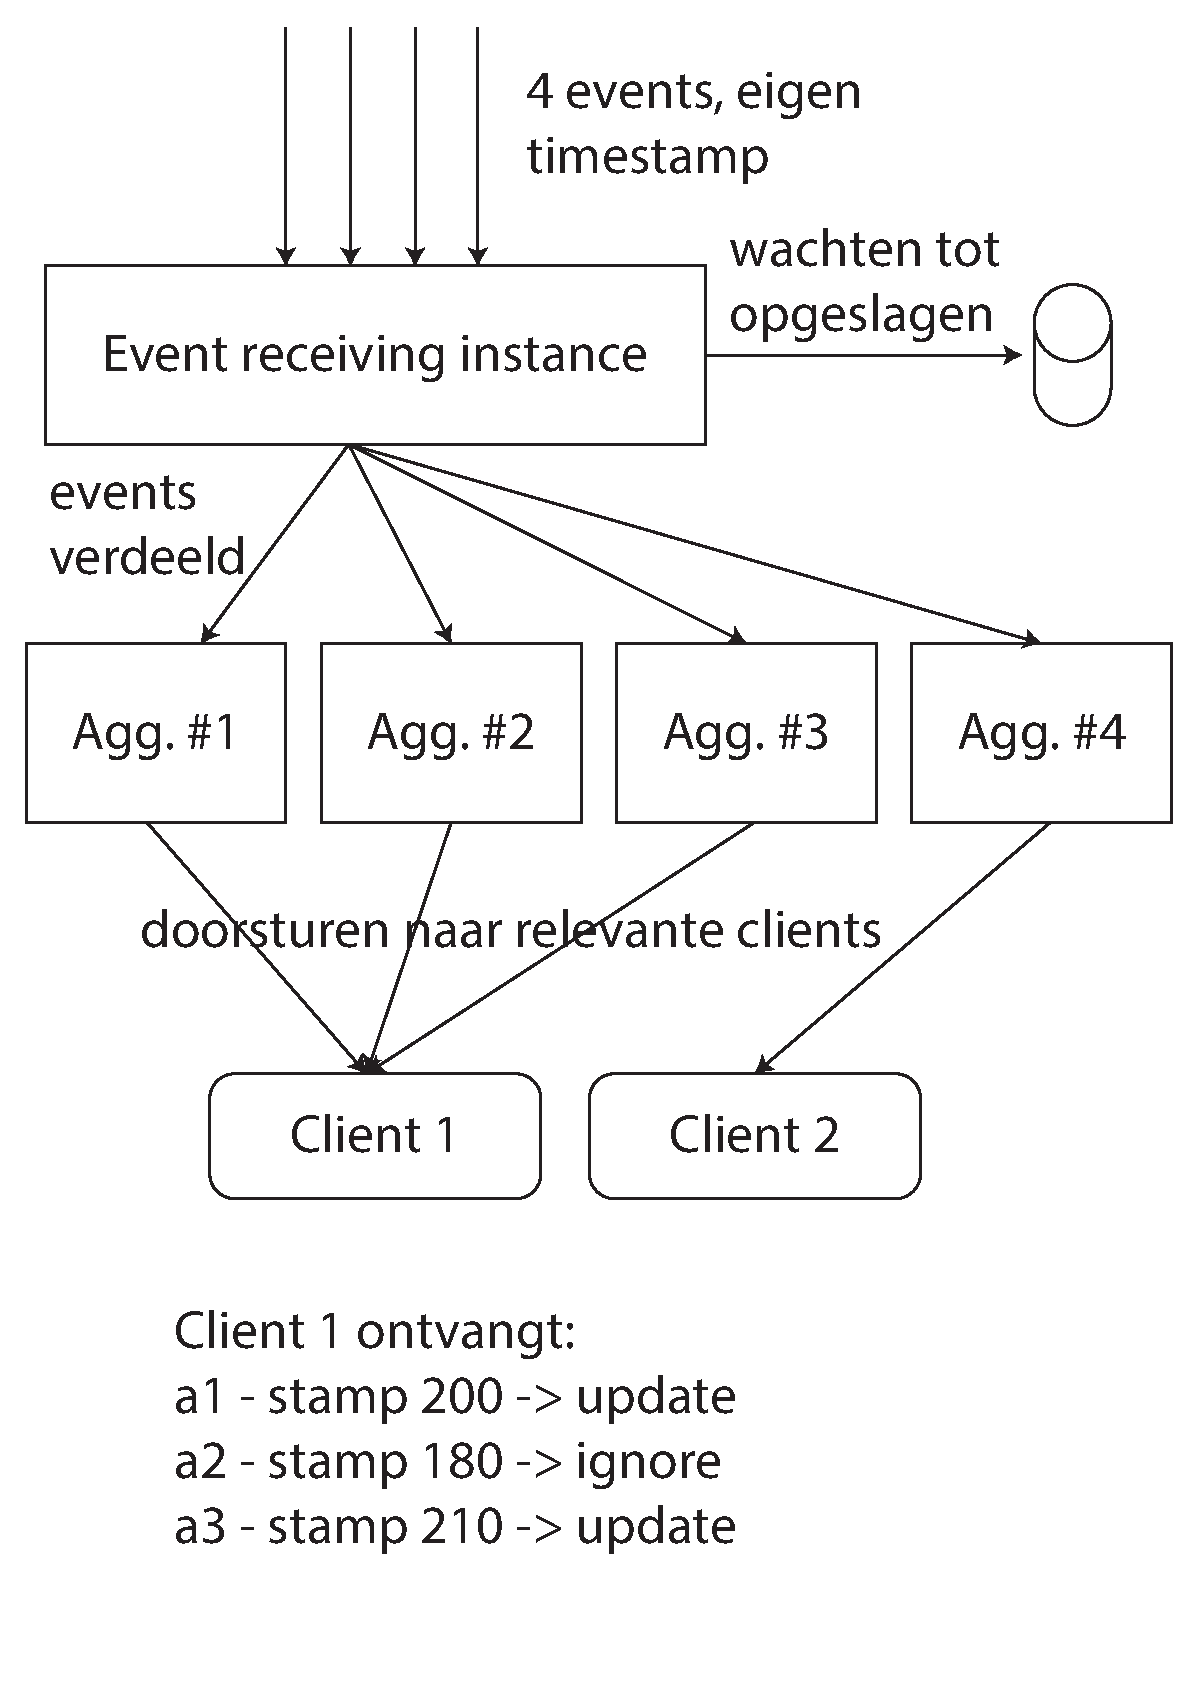
\includegraphics[width=0.4\textwidth]{style/images/meeting1mei}
\caption{Flow bij het binnenkomen van nieuwe Passings}
\label{fig:not1mei}
\end{figure}

\begin{description}
\item[Aggregaties] Aggregaties worden opgeslagen met de timestamp van de laatste Passing die meegenomen is in de berekening. Het doen van de aggregaties kan dus verdeeld worden over meerdere instances, want de laatste Passing die binnenkwam heeft altijd de nieuwste data. De client gebruikt alleen aggregaties met een nieuwe timestamp dan die hij al had. Dit is geschetst en staat in figuur~\ref{fig:not1mei}.

Opslaan van aggregaties kan in Azure Table Store. De partitie id is de (virtuele) groep en de row is de user. De kolommen zijn de verschillende aggregaties. Wanneer er voor een user een nieuwe aggregatie is gedaan worden de normale groepen geupdate en ook de virtuele groepen zoals de aggregatie specifiek voor passings op de specifieke baan waar de laatste passing van binnenkwam.

\begin{table}[h!]
\begin{tabular}{lccccc}
\centering
\textbf{group  } & \textbf{ person } & langste training & snelste ronde & percentage rust/runs \\
\textbf{g1     } & \textbf{ p1     } & 30               & 31            & 10 \\
\textbf{g2     } & \textbf{ p1     } & 31               & 32            & 30 \\
\textbf{g2     } & \textbf{ p2     } & 30               & 30            & 24 \\
\textbf{g3     } & \textbf{ p2     } & 50               & 34            & 60 \\
\textbf{b1     } & \textbf{ p1     } & 32               & 32            & 10 \\
\textbf{b2     } & \textbf{ p1     } & 35               & 30            & 80 \\
\end{tabular}
\label{tab:tablestore} 
\caption{Idee voor aggregatie tabel}
\end{table}

\end{description}

\chapter{Oriëntatieverslag} \label{ch:orientatieverslag} \section{Introductie}

\ifx\aanleiding\undefined
In baansporten is de laatste jaren een ontwikkeling gaande om tijdregistratie te digitaliseren door het gebruik van transponders en detectie-lussen in de baan. Door deze ontwikkeling zijn nieuwe mogelijkheden ontstaan om ook naast het wedstrijdmoment de sportprestaties in te zien. Het constateren van de hierna genoemde nieuwe mogelijkheden was de aanleiding van dit project.

\begin{wrapfigure}{r}{4cm}
  \begin{center}
    \includegraphics[width=4cm]{style/images/transponder}
  \end{center}
  \caption{MyLaps ProFlex transponder, op schaal} 
\end{wrapfigure}
Een grote speler op de tijdregistratie-markt is MyLaps\footnote{\url{http://www.mylaps.com}}. Dit bedrijf installeert en beheert detectie-lussen en is actief bij diverse sporten zoals schaatsen, wielrennen, zwemmen, atletiek en diverse motorsporten. Bij sporten met permanente banen liggen de detectie-lussen het gehele jaar in de baan. Er bestaat de mogelijkheid om op de website van MyLaps doorkomst-tijden in te zien. De informatie die uit deze tijden is af te leiden, wordt door sporters als erg waardevol gezien om zich willen blijven verbeteren, waardoor er steeds meer getraind wordt met deze transponders.

Het huidige gebruik van transponders - buiten wedstrijden - is voornamelijk achteraf, terwijl juist tijdens de training zowel sporter als coach het meeste bezig zijn met de prestaties. Het is daarom wenselijk om de resultaten in real-time door te geven aan coaches en sporters zelf.

Op de banen zijn meerdere detectie-lussen geïnstalleerd, terwijl er op de website van MyLaps slechts 1 wordt ontsloten. In Thialf\footnote{Schaatsbaan in Heerenveen, Friesland; van alle Nederlandse banen wordt deze baan het meeste gebruikt voor professionele wedstrijden.} liggen bijvoorbeeld 12 detectie-lussen en op de andere schaatsbanen liggen er tenminste 2. Door de data van meerdere lussen te combineren is een betere indicatie te maken van de snelheid van sporters. Veel trainingselementen bestaan uit korte opdrachten, waar het juist om snelheid gaat. Een enkele lus is dan niet afdoende, omdat de rust voor of na de opdracht mee wordt gewogen. Wanneer er op tactische punten detectie-lussen geïnstalleerd zijn, is er bijvoorbeeld ook onderscheid te maken tussen bochten en de rechte stukken. Bij sporten met een ronde baan verschilt de snelheid in de bocht namelijk erg met die op het rechte eind. Deze vergelijking gebeurt nu al in Thialf, in het professionele circuit.

Topsporters zijn enorm prestatiegericht en als je al aan de top zit, dan kunnen kleine aanpassingen aan je techniek, ademhaling et cetera, grote verschillen maken. Coaches van professionele teams houden zich daarom bezig met allerhande analyses. Naast ademanalyse en hartslag monitoring, is het in Thialf bijvoorbeeld ook mogelijk om (van maximaal 20 schaatsers) continu de positie te bepalen met een in-door positioning system (IPS) ontwikkeld door InnoSportLab\footnote{\url{http://www.innosportlabthialf.nl}}.

Al deze geavanceerde analyses zijn te duur en kosten te veel tijd voor recreatieve sporters. MyLaps X2 biedt in combinatie met ons eindproduct recreatieve sporters toch een manier om analyses uit te voeren en zich naar een hoger niveau te tillen.
\fi

Aan de hand van de projectopdracht, ons Plan van Aanpak (te vinden in Appendix~\ref{ch:plan-van-aanpak}) en gesprekken met Johan en Cor-Paul hebben we dit Ori\"entatieverslag opgesteld. Dit verslag biedt inzicht in de mogelijke technieken voor het ontwikkelen van mobiele applicaties en server back-ends, geschikt voor onze toepassing. Ook zullen in dit verslag de keuzes voor het gebruik van bepaalde technieken worden toegelicht.

\section{Back-end}\label{sec:orientatie-back-end}
Afhankelijk van welk back-end platform we kiezen, zijn er verschillende mogelijkheden voor de servers waarop de back-end kan draaien. Ook is er de keuze tussen traditionele server clusters en een cloud-oplossing, zoals een \ac{paas}. Er zijn verschillende redenen om wel of niet voor een cloud oplossing te gaan. De voor- en nadelen van een cloud oplossing staan hieronder opgesomd.
\begin{itemize} 
    \item[+] Automatisch en vrijwel onbeperkt schaalbaar
    \item[+] Opzetten besturingssysteem is niet nodig
    \item[+] Geen onderhoud nodig
    \item[+] Gegarrandeerde hoge uptime
    \item[-] Mogelijk duurder vanwege winstmarge \ac{paas}
    \item[-] Minder keuze in hoeveelheid beschikbare talen/frameworks
\end{itemize}

\begin{table}
\begin{tabular}{lccccc}
\textbf{}        & \multicolumn{1}{l}{\textbf{Azure}} & \multicolumn{1}{l}{\textbf{App Engine}} & \multicolumn{1}{l}{\textbf{AWS}} & \multicolumn{1}{l}{\textbf{Heroku}} & \multicolumn{1}{l}{\textbf{AppFog}} \\
\textbf{.NET}    & \times &        & \times &         &        \\
\textbf{Java}    & \times & \times & \times & \times  & \times \\
\textbf{Scala}   & \times & \times & \times & \times  & \times \\
\textbf{Python}  & \times & \times & \times &         & \times \\
\textbf{Node.JS} & \times &        & \times & \times  & \times \\
\textbf{PHP}     & \times & \times & \times &         & \times \\
\textbf{Ruby}    & \times &        & \times & \times  & \times \\
\textbf{Overig}  &        & Go     &        & Closure & Erlang
\end{tabular}
\caption {Vijf grote \ac{paas} providers en de talen en frameworks die ze ondersteunen} \label{tab:paas} 
\end{table}

Het nadeel dat de prijs hoger kan liggen kan worden afgezwakt en mogelijk worden omgebogen: om grote hoeveelheden gebruikers aan te kunnen moet een traditioneel server cluster groot zijn, terwijl een \ac{paas} automatisch kan schalen en dus op dal-momenten significant goedkoper kan zijn. We verwachten dat het gebruik van onze applicatie een piek zal vertonen in de avond en in het weekend, omdat er voornamelijk buiten werk en schooltijd gesport wordt. Er is voor onze applicatie dus meer dal- dan piek-belasting en we verwachten dus ook dat een \ac{paas} oplossing goedkoper zal zijn dan een cluster.

In tabel~\ref{tab:paas} ziet u een overzicht van de verschillende grote cloud platformen die er momenteel zijn, en de talen en frameworks die ze ondersteunen~\cite{paas-list-tomsitpro, azure-scala, aws}. Zoals in de tabel te zien is ondersteunen de meeste \ac{paas}\'s vele talen en frameworks. Microsoft Azure en Amazon AWS ondersteunen de 4 grote platformen .NET, Java, Python en NodeJS.

De bestaande systemen van Emando zijn gemaakt met het .NET framework en draaien voornamelijk in Microsoft Azure als Cloud Service. Aangezien MyLaps voor ons een belangrijke databron is en de MyLaps SDK alleen voor C\#/.NET beschikbaar is, kan er veel werk bespaard worden door ook deze programmeertaal en runtime te gebruiken. 

Bovendien heeft Emando een laag over de MyLaps SDK heen geschreven waardoor de SDK bruikbaar is met \acf{rx}. \ac{rx} - mede ontwikkeld door prof.dr. H.J.M. Meijer~\cite{meijer2011world} - is een manier om LINQ te gebruiken voor observeerbare collecties en asynchroon programmeren, twee eigenschappen waar we binnen de applicatie mee te maken gaan krijgen.

Bij onze keuze hebben ook de andere platformen overwogen, maar door de beperkte beschikbaarheid van de MyLaps SDK (alleen binnen .NET) en het gebruik van .NET door Emando waren dit minder bruikbare opties.

\subsection{Real-time}\label{sec:orientatie-real-time}
De trainingsapplicatie moet zonder dat de gebruiker de applicatie handmatig ververst de laatste doorkomsten binnenkrijgen en tonen. Ook moet de getoonde rondetijd up to date zijn, en niet een ronde tijd van een vorig rondje. De communicatie tussen de back-end en de clients moet dus real-time zijn. Real-time wil zeggen dat de server een update naar de client kan sturen. In `normaal' web verkeer kan de server niet op elk moment een bericht sturen naar de client. De server kan alleen reageren op een verzoek van de client, omdat de client geen vast IP-adres heeft en er standaard geen poort open staat. Pas wanneer de client een uitgaand verzoek heeft gaat er een poort open.

Een oplossing hiervoor is WebSockets: bij WebSockets blijft de verbinding open en dus de poort en kan de server op elk moment een bericht sturen, als er bijvoorbeeld een schaatser voorbij een detectie-lus komt. Een verbinding openhouden kost geheugen op de server en de server heeft dus een maximum aantal verbindingen dat hij kan openhouden. Er bestaan verschillende WebSocket frameworks die je het aanmaken en onderhouden van de verbindingen uit handen nemen. Een hiervan is SignalR voor .NET. Emando heeft SignalR\footnote{http://www.asp.net/signalr} succesvol gebruikt tijdens de Olympische Spelen van 2014 om \url{http://live.schaatsen.nl} te voorzien van live data. SignalR is inmiddels een officiele ASP.NET library en wordt ontwikkeld en ondersteund door Microsoft ontwikkelaars.

\section{Client}
Er zijn tegenwoordig diverse manieren om mobiele applicaties te maken, voor diverse platformen (iOS, Android, Windows Phone). Deze verschillende methodes vereisen verschillende programmeertalen en architecturen. Een groot verschil tussen de verschillende methodes is de hoeveelheid code die kan worden hergebruikt tussen verschillende platformen. De uitersten hiervan gebruiken een compleet gescheiden broncode ten opzichte van een volledig gedeelde broncode. De volgende methodes zijn meegenomen in onze ontwerpkeuze:

\begin{description}
\item[Native applicatie:] Een native applicatie is een applicatie die ontworpen is voor een specifiek platform. Het design van dergelijke applicaties ligt (meestal) in het verlengde van de richtlijnen voor dit platform en het gebruik van platform specifieke handelingen (gestures) wordt gestimuleerd en gehanteerd binnen de applicatie. Vanwege de richtlijnen en het gebruik van deze gestures, zijn dergelijke applicaties zelfverklarend voor eindgebruikers. Een ander voordeel is dat door de native implementatie, de user interface performance van dergelijke applicaties doorgaans erg goed is.

Een nadeel van native applicaties is dat applicatie code vaak in een platform specifieke programmeertaal wordt ontwikkeld en dat er daardoor 3 complete applicaties ontwikkeld moeten worden om de drie grootste platformen te ondersteunen (iOS, Android en Windows Phone). Het ontwikkelen hiervan kost daardoor vaak veel tijd.
    
\item[Web applicatie:]
Een web applicatie is een applicatie die ontworpen is om op alle (mobiele) platformen te draaien. Deze applicatie is benaderbaar via het web (m.b.v. browsers) en heeft als groot voordeel dat deze maar 1x ontwikkeld hoeft te worden. Ook zijn veel ontwikkelaars bekend met de programmeertalen waarmee gewerkt moet worden (HTML, CSS en JavaScript).
    
Er zijn veel verschillende frameworks om mobiele applicaties te maken en daar ligt ook meteen een groot gevaar: elk framework heeft zijn eigen voordelen en wisselen tussen frameworks kan vaak betekenen dat grote delen van de applicatie opnieuw geschreven moeten worden. Ook tijdens ons project zijn diverse frameworks (Meteor, Angular, Backbone, Ember) ter sprake gekomen en voor elk genoemd framework wist er een projectlid voor- en nadelen te noemen.
    
\textbf{Frameworks:} jQuery Mobile~\cite{jq-mobile}, Sencha Touch~\cite{sencha}, Meteor~\cite{meteor}, AngularJS~\cite{angular}, Backbone.js~\cite{backbone}, Ember.js~\cite{ember}, Ionic~\cite{ionic}, React~\cite{React}
    
\item[Native applicatie met WebView:] Een ander belangrijk nadeel van web applicaties is het feit dat deze niet vindbaar zijn in de app stores. Native applicaties met een WebView\footnote{Een WebView is een soort van browser binnen een applicatie, zonder de mogelijkheid zelf een url in te voeren.} zijn applicaties waarin met behulp van een webview een reeds bestaande web applicatie geladen wordt. Hiermee kan met relatief weinig tijd worden meegeleund op het model van de applicatie winkels en is de applicatie in een klap vindbaar op de plek waar gebruikers zoeken naar applicaties.
    
Een nadeel van deze applicaties is hun performance. De applicatie laadt steeds webpagina's in en bij het wegvallen van de verbinding kan de applicatie doorgaans geen of weinig informatie of user interface tonen. Ook kan er doorgaans geen of weinig gebruik gemaakt worden van gestures. In sommige implementaties van deze applicaties wordt een onderscheid gemaakt tussen de offline user interface en de online web app, wat de performance verbetert en het probleem met het wegvallen van de verbinding oplost. De prestaties, vormgeving en gestures zijn echter vele malen minder praktisch ingericht dan bij een native applicatie. Het uitbrengen van een applicatie binnen de applicatie winkels brengt echter wel verwachtingen met zich mee. Doorgaans gaan gebruikers er vanuit dat de bovenstaande beschreven eigenschappen wel verwerkt zitten binnen deze applicaties.   
\textbf{Frameworks:} PhoneGap/Cordova~\cite{cordova}, Titanium~\cite{titanium}
    
\item[Cross Compiling: ] Cross Compiling is een techniek om broncode om te zetten naar uitvoerbare bestanden voor de verschillende platformen. Hiermee kan vaak de business- en servicelaag van de applicatie gedeeld worden tussen platformen, en sommige `cross-compilers' ondersteunen ook het delen van de presentatielaag. Vaak is dit echter niet wenselijk, omdat juist op de presentatielaag veel verschil gemaakt kan worden tussen platformen, om beter aan te sluiten bij de verwachtingen van de gebruiker. Met cross compiling wordt tijd bespaard op de business- en servicelaag, welke gebruikt kan worden om een presentatielaag te maken voor meerdere platformen. Applicaties die gemaakt zijn door middel van Cross Compilation zijn niet te onderscheiden van native applicaties (gemaakt in de programmeertaal van het platform) want de uitvoerbare bestanden zijn binair vrijwel gelijk.
    
Een nadeel van Cross Compiling is dat het opzetten van de architectuur direct op een juiste manier dient te gebeuren, hetgeen tijd extra tijd kan kosten. Het later aanpassen van de architectuur heeft tot gevolg dat er voor alle platformen een update nodig is voordat het project weer succesvol compileert. Ook moet er in tegenstelling tot een web app nog steeds voor meerdere platformen ontwikkeld worden.
    
\textbf{Frameworks:} Xamarin~\cite{xamarin}, Adobe AIR~\cite{adobeair}, XMLVM~\cite{xmlvm}, Apportable~\cite{apportable}
\end{description}

\subsection{Xamarin}
Wisselen tussen methodiek betekent het opnieuw ontwikkelen van de applicatie. Omdat onze applicatie niet alleen een proof-of-concept is, maar bedoeld is voor echt gebruik en doorontwikkeling, is het economisch voordeliger om direct voor de uiteindelijke methodiek te kiezen.
    
Omdat performance en responsetijd een belangrijke rol spelen binnen onze applicatie, ligt het voor de hand om voor een native of gelijkwaardig presterende aanpak te gaan. Een implementatie met WebView biedt niet de performance waar we naar op zoek zijn.
    
In overleg met de opdrachtgever is besloten de applicatie te ontwikkelen voor \'e\'en platform met een Cross Compiling-implementatie. Het ontwikkelen van deze applicatie (met de gestelde eisen) voor meerdere platformen kost meer tijd dan ontwikkelen voor een enkel plaftform, en zou ten koste gaan van het \ac{mvp}. Door een goede business- en servicelaag op te zetten, is het later mogelijk om de applicatie uit te rollen naar andere platformen, door enkel de platform specifieke views nog te ontwikkelen.

We hebben voor Xamarin boven andere Cross Compiling implementaties gekozen omdat Xamarin werkt met het .NET framework,vanwege de .NET SDK van MyLaps en de .NET implementaties van Emando.Dit brengt een paar belangrijke voordelen met zich meebrengt:

\begin{itemize}
    \item Het platform .NET biedt LINQ en \acf{rx}. Met LINQ en \ac{rx} kunnen eenvoudig streams aan binnenkomende data efficient afgehandeld worden. Aangezien dit een belangrijk onderdeel is van onze applicatie is dit een groot voordeel.
    \item Aangezien we onze server zullen inrichten met SignalR is het fijn dat er al een SignalR component bestaat voor Xamarin. Dit maakt de communicatie met de server een `no-brainer'.
    \item Emando gebruikt \acf{tfs} en de integratie van Xamarin met Visual Studio (en daarmee \ac{tfs}) zal latere doorontwikkeling en aansluiting op de bestaande werkwijze ten goede zou komen.
\end{itemize}

\subsection{iOS}
Vanwege de projectduur is besloten de applicatie aanvankelijk voor slechts 1 platform uit te rollen en dusdanig in te richten zodat deze later gemakkelijk uitgebreid kan worden naar andere platformen. 

Omdat er voor slechts één platform een applicatie uitgerold wordt, is de keuze voor dit platform niet onbelangrijk. Het kiezen voor het platform is gebeurd aan de hand van de volgende criteria:
\begin{itemize}
\item Aantal schaatsers die het platform gebruiken
\item Moeilijkheidsgraad om naar platform uit te rollen
\end{itemize}

De moeilijkheidsgraad om naar een specifiek platform uit te rollen bleek bij alle platformen nagenoeg even hoog. Platformen als \textit{Windows Phone}\footnote{http://www.windowsphone.com/} en \textit{BlackBerry}\footnote{http://www.blackberry.com} hebben niet genoeg market share en aantal gebruikers om het uitrollen van de applicatie rendabel te maken. \textit{Android}\footnote{http://www.android.com/} en \textit{iOS}\footnote{http://www.apple.com/nl/ios/} hebben een grote market share en veel actieve gebruikers. Van de medewerkers van de schaatsbond beschikt de meerderheid over een mobiel aparaat dat \textit{iOS} draait, hetgeen de doorslaggevende factor is geweest om aanvankelijk de applicatie eerst voor \textit{iOS} te ontwikkelen.

\section{Entiteiten}
De data binnen onze applicatie bestaat uit verschillende entiteiten. In figuur~\ref{fig:entities} is de relatie tussen de entiteiten afgebeeld. De entiteit op het kleinste niveau is \textit{Passing}, de doorkomst bij een detectie-lus. Een doorkomst heeft velden voor het moment van registratie, welke lus detecteerde, welke baan de lus staat en welke transponder er bij hoort. Passings komen uit de MyLaps SDK en zijn dus externe data, die we wel zelf moeten opslaan. De MyLaps SDK is namelijk niet bedoeld als database om Passings te selecteren, maar slechts om real-time Passings te verkrijgen.

\begin{figure}
\centering
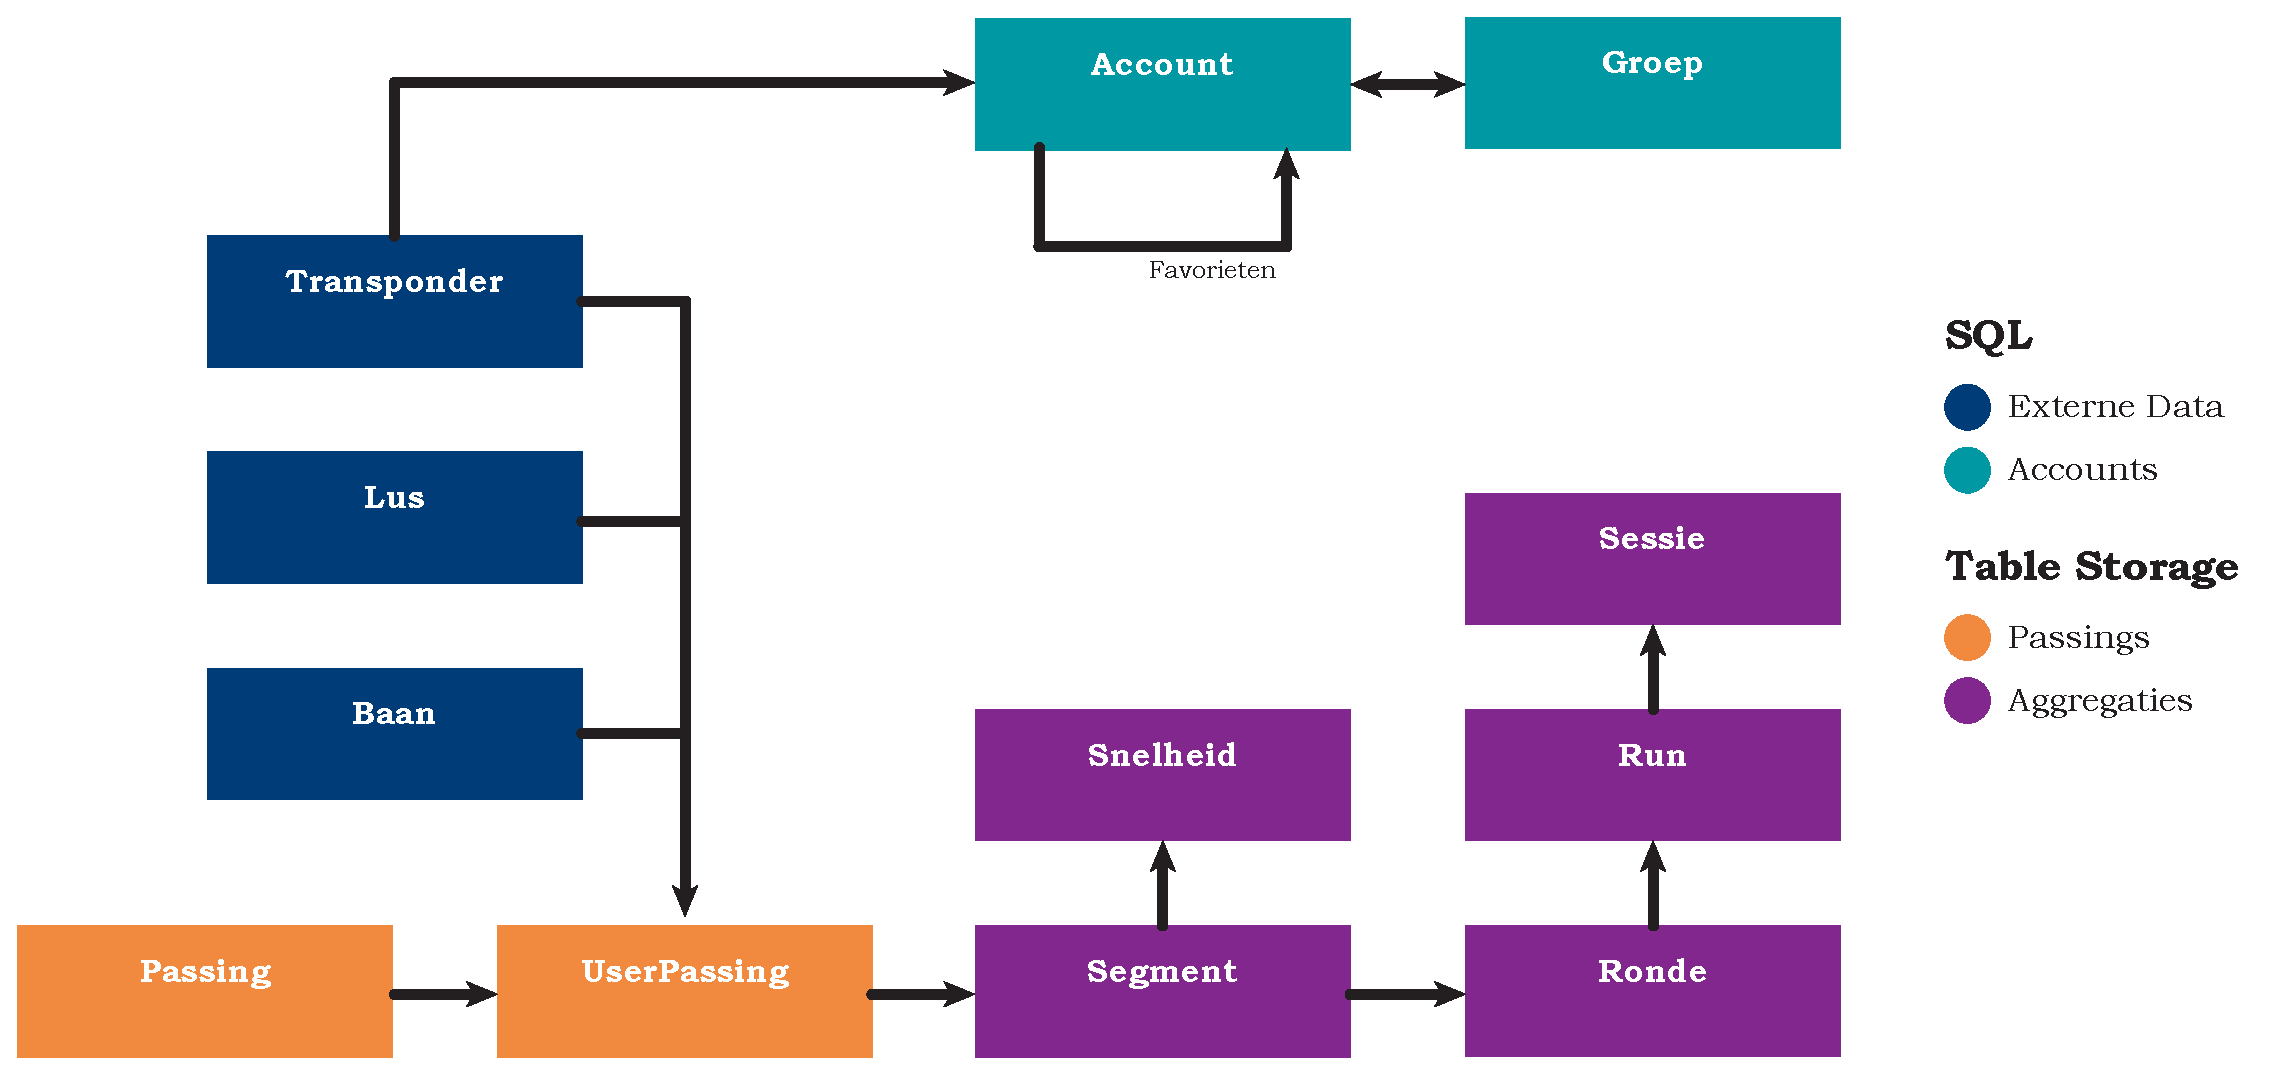
\includegraphics[width=0.8\textwidth]{style/images/Entiteiten}
\caption{Entiteiten binnen de applicatie}
\label{fig:entities}
\end{figure}


Wanneer een Passing ons systeem binnenkomt proberen we deze te koppelen aan een gebruiker. Als Passing bij een voor ons onbekende transponder hoort slaan we de Passing op en verwerken we hem later, als we de betreffende transponder wel kennen. Dit kan gebeuren als een gebruiker met terugwerkende kracht een transponder koppelt aan zijn account. Elke gebruikersaccount heeft dus een lijst met transponders en vanaf wanneer tot wanneer deze transponder in het bezit van de gebruiker was. Een transponder kan namelijk ook worden uitgeleend. Per tijdseenheid kan er per gebruiker maar één transponder zijn.

Aan de hand van een lijst met Passings kunnen we enkele berekeningen doen. Met deze berekeningen kunnen we bijvoorbeeld bepalen wanneer een training begint en eindigt. Een groep van de Passings van een training heet een Session. Binnen een training zijn weer Runs te onderscheiden. Runs zijn groepjes van passings waartussen een sporter niet uitreed. Een training in het baansporten kan er bijvoorbeeld bestaan uit het 5 keer rijden van 4 ronden, met tussendoor 2 ronden rust. Er zijn in dat geval binnen de sessie 4 runs te onderscheiden. In figuur~\ref{fig:sessions} is een training van Herman te zien. Bij Herman zijn rondetijden langzamer dan 40 seconden  geen actieve onderdelen, maar zijn uitrijd-rondjes. Dit is per sporter en sport verschillend, dus moet deze grens dynamisch bepaald worden of instelbaar zijn. In de figuur zijn de runs groen gekleurd.

\begin{figure}
\centering
\includegraphics[width=1\textwidth]{style/images/MyLapsHerman}
\caption{De rondetijden tijdens een typische training; specifiek: training van Herman van 3 maart 2014}
\label{fig:sessions}
\end{figure}

\section{Database}
Uit figuur~\ref{fig:entities} blijkt dat een deel van onze data relationeel is. De gebruikers zijn gekoppeld aan transponders en transponders zijn gekoppeld aan Passings. Gebruikers kunnen deel uitmaken van groepen en kunnen een lijst met favoriete gebruikers hebben, welke ze willen volgen. Een deel van de data zullen we opslaan in een relationele database. Data die relatief weinig wordt aangepast zoals de gebruiker-accounts en bijbehorende transponders leent zich hier uitstekend voor. Met een \textit{join} is eenvoudig een lijst van transponders van een gebruiker op te halen. In figuur~\ref{fig:dbengines} is (een abstractie en deel van) de relationele data weergegeven in het blauw. De user-id's uit de account-tabel komen terug in de transponder-tabel.

\begin{figure}
\centering
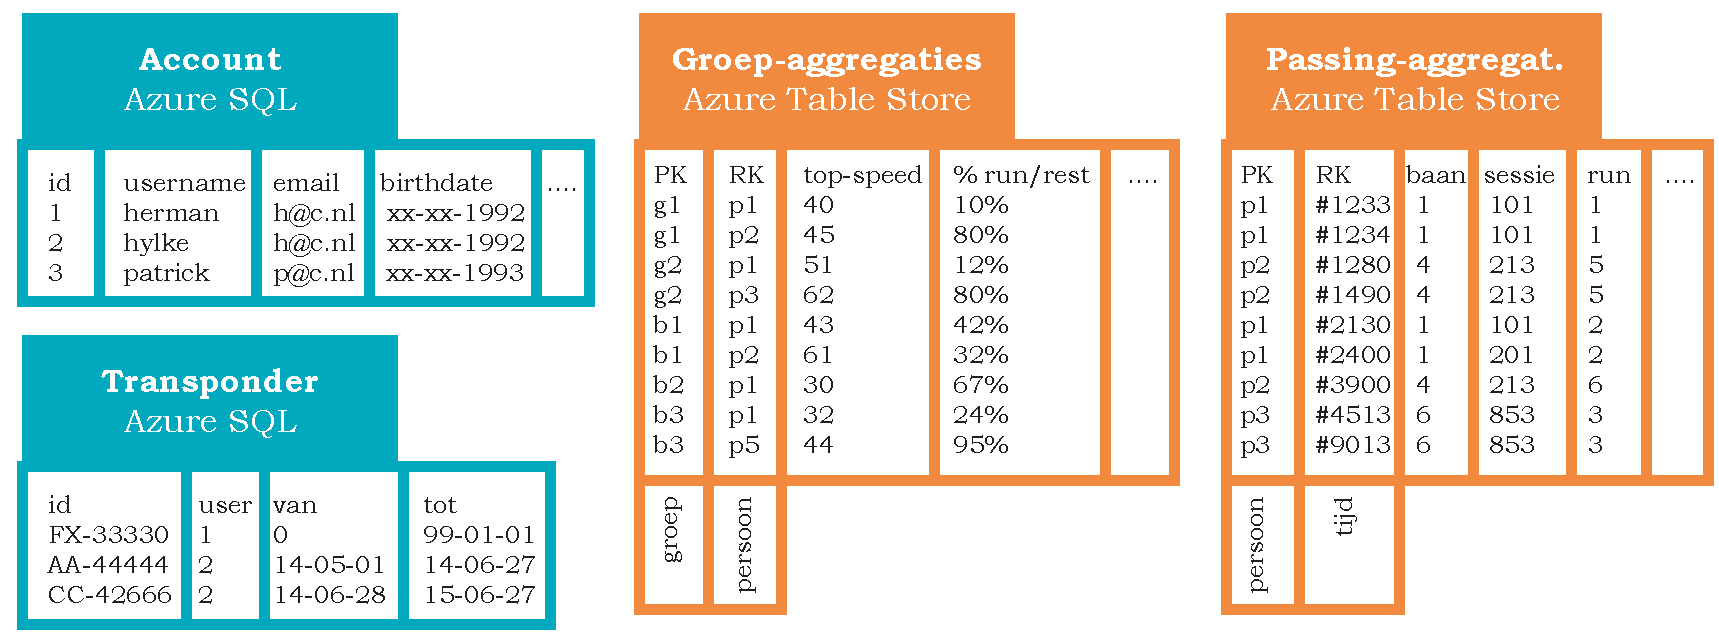
\includegraphics[width=\textwidth]{style/images/DBEngines}
\caption{Verschillende data, verschillende database engines}
\label{fig:dbengines}
\end{figure}

Naast de relationele data, genereren we met aggregaties heel veel platte data, zoals de snelste rondetijd, de langste run, of de hoogste snelheid per persoon. Deze data is gebonden aan de groepen waarin een gebruiker zit en de banen waarop de Passing plaatsvond. In de meeting van 1 mei (Appendix~\ref{sec:meeting-1-mei}) is besproken om hiervoor de Azure Table Storage te gebruiken. Table Storage heeft twee keys per rij, de PartitionKey en de RowKey~\cite{azuretablestorage}. Wij slaan de (virtuele) groep op in de PartitionKey (PK) en de gebruikers in de RowKey (RK). Op die manier is snel voor een groep alle data op te halen, voor bijvoorbeeld een Leaderboard. Ook kan bij het opslaan van de aggregaties snel op de RowKey gefilterd worden. De verschillende aggregaties worden opgeslagen in verschillende kolommen. Azure Table Storage biedt de namelijk mogelijkheid arbitraire objecten te koppelen aan een PartitionKey en RowKey (de combinatie van de twee keys is uniek). In figuur~\ref{fig:dbengines} is (abstractie van) de platte data weergegeven in het oranje. In de Passing aggregatie tabel is de unieke key gebaseerd op de transponder en de timestamp van de Passing. Een transponder kan niet twee keer gedetecteerd worden op hetzelfde moment zonder dat het dezelfde Passing is. Aggregaties per passing zoals bij welke run en sessie de Passing hoorde slaan we hier in op.

Deze data wordt real-time verwerkt en doorgestuurd naar de client wanneer nodig. Om deze aggregaties snel en onafhankelijk van elkaar te laten verlopen, moet rekening worden gehouden met de mogelijkheid om bij pieken meerdere instanties van deze aggregatie-pijpen te draaien. Elke instantie ontvangt dan andere Passings. Om te zorgen dat de client altijd de laatste versie ontvangt wordt elke aggregatie vergezeld van de \textit{timestamp} van de laatste Passing. Als een client een aggregatie ontvangt met een oudere timestamp dan degene die hij al ontvangen heeft dan kan hij deze negeren.

\section{Architectuur}
In overleg met de opdrachtgever is gekozen voor een multi-layered architectuur met
vier lagen: de data-laag, business-laag, service-laag en de presentatie-laag. Deze 
architectuur garandeert een scheiding tussen verschillende stukken logica, zodat 
alle logica in de verantwoordelijke laag wordt uitgevoerd. In Figuur~\ref{fig:architecture} zijn alle layers en hun componenten weergegeven.

\begin{figure}
\centering
\includegraphics[width=\textwidth]{style/images/Architectuur}
\caption{Systeem architectuur}
\label{fig:architecture}
\end{figure}

De data-laag bevat componenten die een  verbinding kunnen maken met de databases en 
andere services zoals MyLaps Cloud en de Facebook API. De data-laag zet ruwe data 
uit de database om in domein entiteiten en levert deze af bij de business-laag.

De business-laag bevat alle workflows die op de server uitgevoerd moeten worden. 
De workflows zijn in drie categorieen op te delen. Als eerste de Aggregatie
componenten die diverse aggregaties kunnen uitvoeren op data uit de Practice
Database. Ten tweede is er de Event Workflow die bepaald wat er moet gebeuren als
er een event binnenkomt zoals bijvoorbeeld een doorkomst vanaf MyLaps. In het
geval van een doorkomst moet deze bijvoorbeeld worden opgeslagen in de Practice
Database en moeten de aggregaties een iteratie doorlopen. Als derde is er het User
Account component dat acties voor gebruikersacccounts mogelijk maakt. Zo is dit
component belast met het opslaan van nieuwe users, het inloggen met wachtwoord of
met Facebook, het beheren van groepen en het ophalen van vriendenlijsten.

De service-laag bevat de API. De diverse aanroepen die de clients nodig hebben
worden in de service-laag gekoppeld aan de goede workflow uit de business-laag. De
service-laag zorgt ook voor Caching, waar nodig.

De presentatie-laag bevindt zich in de mobiele applicaties. Deze toont de informatie uit de
service-laag. De presentatie-laag bevat bijvoorbeeld User Interface componenten, 
weergaves voor diverse data types en menu's. Naast de weergave zit er in de apps 
ook een stuk service-laag om te kunnen communiceren met de service-laag op de 
server.

\chapter{Interface Ontwerpen} \label{ch:interface-ontwerpen} \begin{figure}[ht]
\centering
\subfigure[Beginscherm]{
    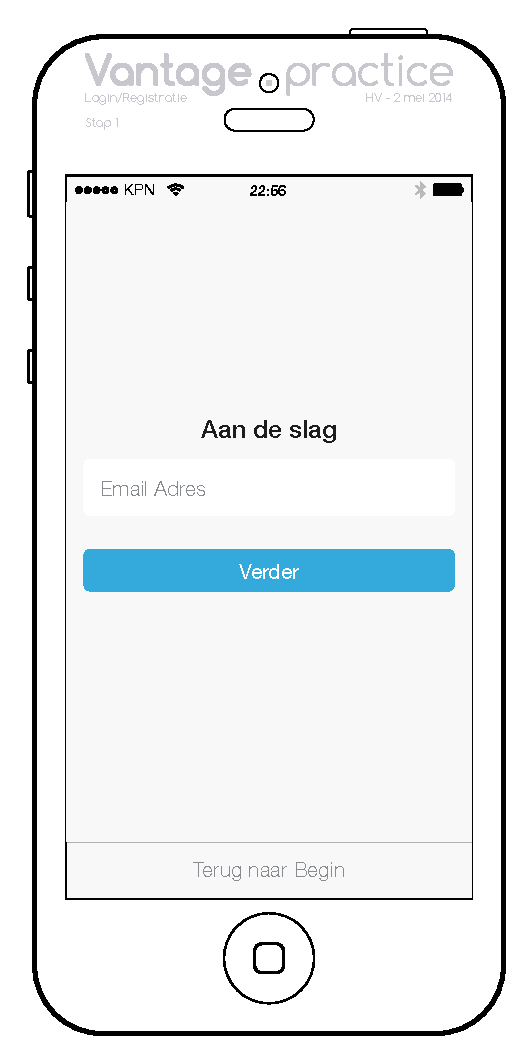
\includegraphics[width=4.5cm]{style/images/designs/02-A-Login-Registratie}
    \label{fig:login-registratie}
}
\subfigure[Registratiescherm]{
    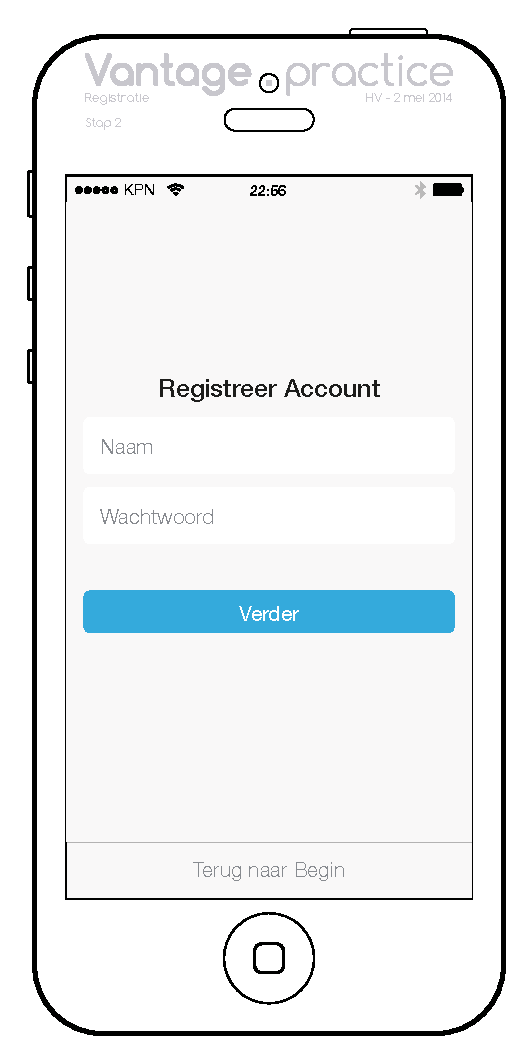
\includegraphics[width=4.5cm]{style/images/designs/02-B1-Registratie}
    \label{fig:registratie}
}
\subfigure[Loginscherm]{
    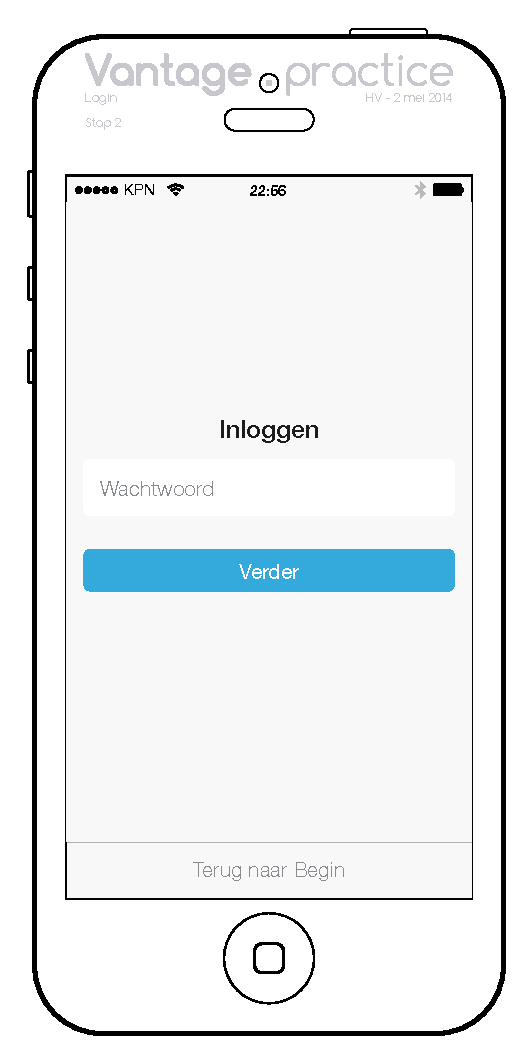
\includegraphics[width=4.5cm]{style/images/designs/02-B2-Inloggen}
    \label{fig:login}
}
\caption{Login en registratie}
\label{fig:login-en-registratie}
\end{figure}

\begin{figure}[ht]
\centering
\subfigure[Profielscherm]{
    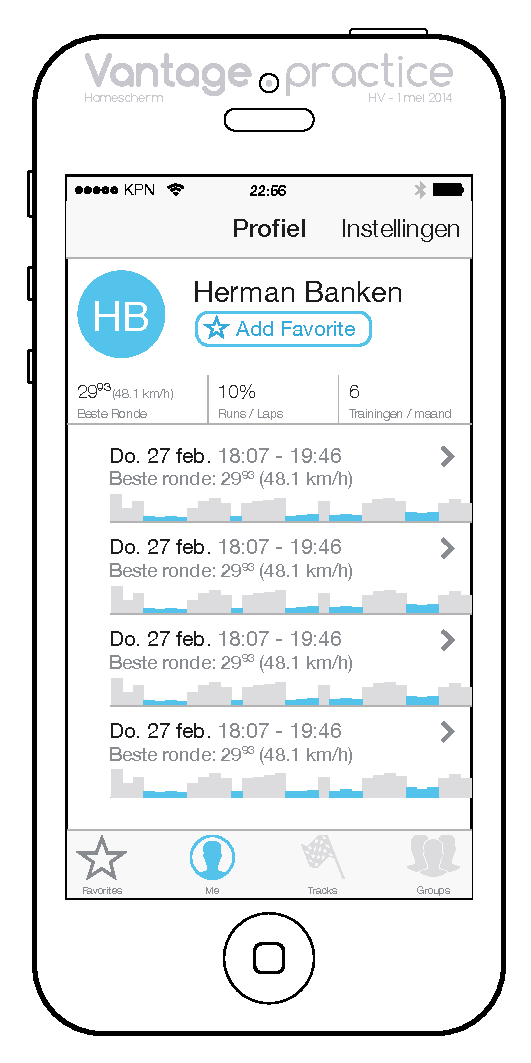
\includegraphics[width=4.5cm]{style/images/designs/03-Home}
    \label{fig:home}
}
\subfigure[Accountinstellingen]{
    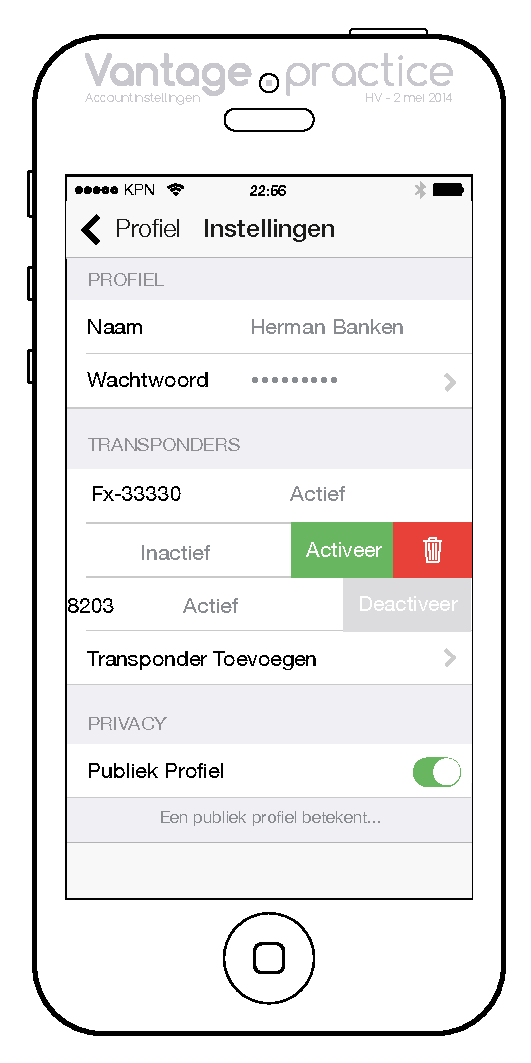
\includegraphics[width=4.5cm]{style/images/designs/04-A-Accountinstellingen}
    \label{fig:accountinstellingen}
}
\subfigure[Transponder Toevoegen]{
    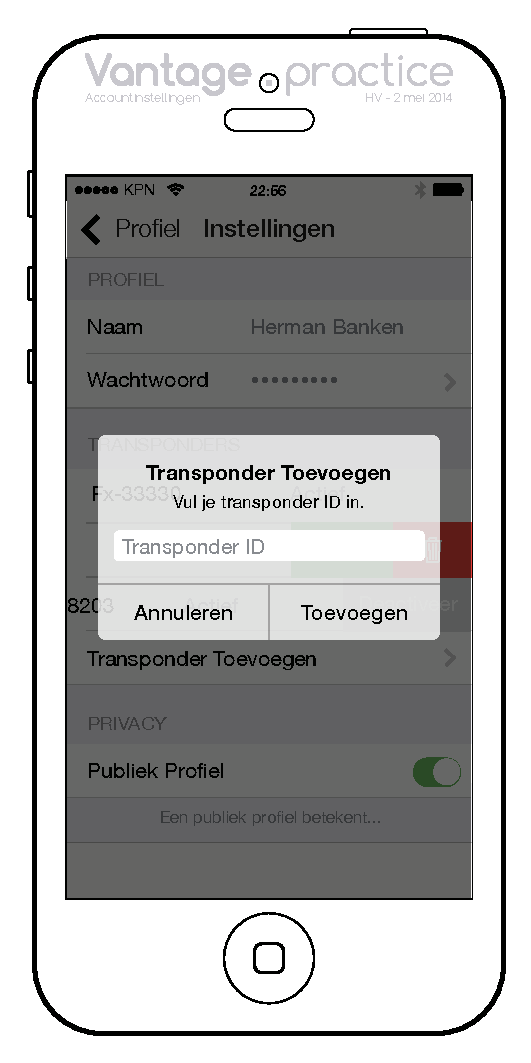
\includegraphics[width=4.5cm]{style/images/designs/04-B-Transponder_Toevoegen}
    \label{fig:transponder-toevoegen}
} % In de download ziet het er wel goed uit!
\caption{Profiel en accountinstellingen}
\label{fig:profiel-en-accountinstellingen}
\end{figure}

\begin{figure}[ht]
\centering
\subfigure[Sessieoverzicht]{
    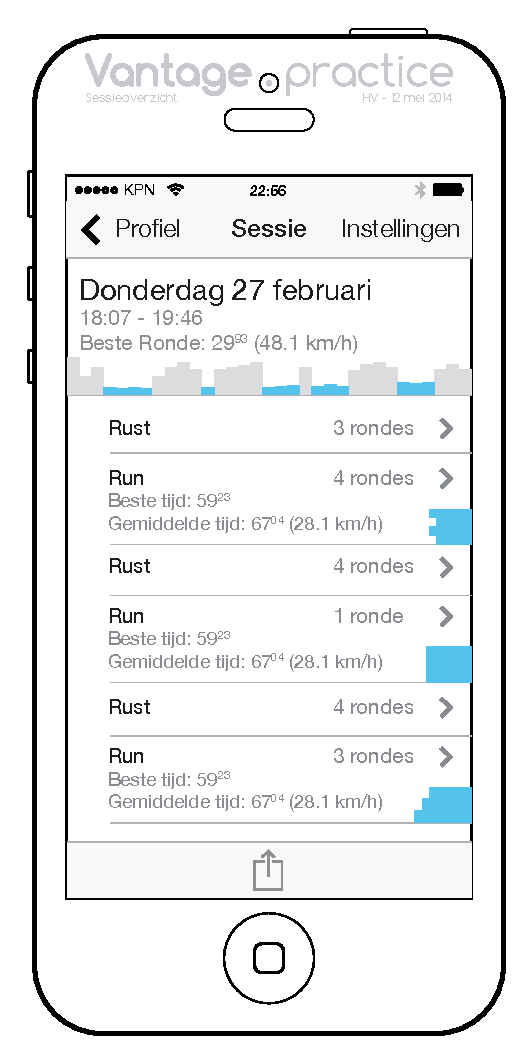
\includegraphics[width=4.5cm]{style/images/designs/06-Sessieoverzicht}
    \label{fig:ingeklapt-sessieoverzicht}
}
\subfigure[Sessieoverzicht met een opengeklapte run]{
    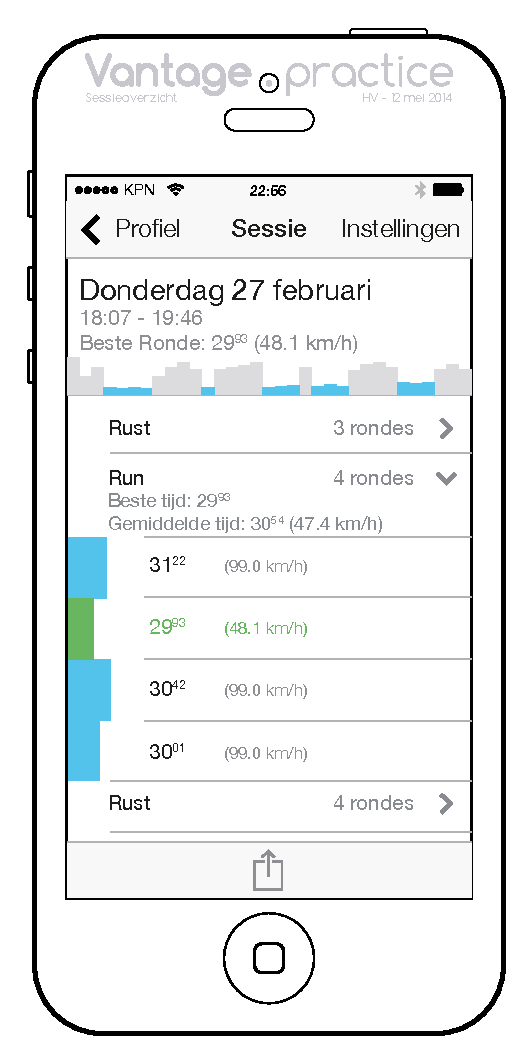
\includegraphics[width=4.5cm]{style/images/designs/07-Runoverzicht}
    \label{fig:uitgeklapt-sessieoverzicht}
}
\caption{Sessie-schermen}
\label{fig:sessie-schermen}
\end{figure}

\begin{figure}[ht]
\centering
\subfigure[Favorietenoverzicht]{
    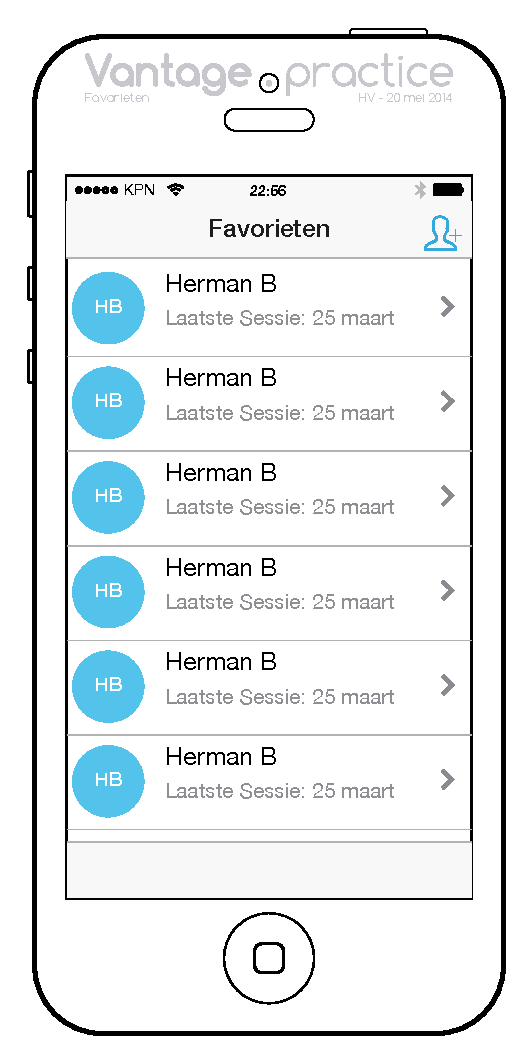
\includegraphics[width=4.5cm]{style/images/designs/09-Favorieten-A}
    \label{fig:favorieten-lijst}
}
\subfigure[Favorieten Toevoegen]{
    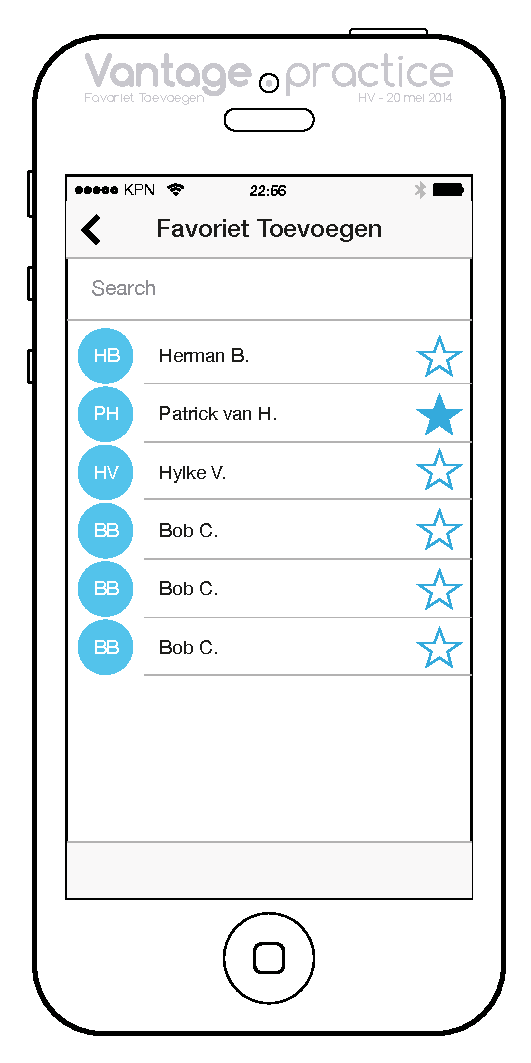
\includegraphics[width=4.5cm]{style/images/designs/09-Favorieten-B}
    \label{fig:favorieten-toevoegen}
}
\caption{Favorieten-schermen}
\label{fig:favorieten-schermen}
\end{figure}

\begin{figure}[ht]
\centering
\subfigure[Groepenoverzicht]{
    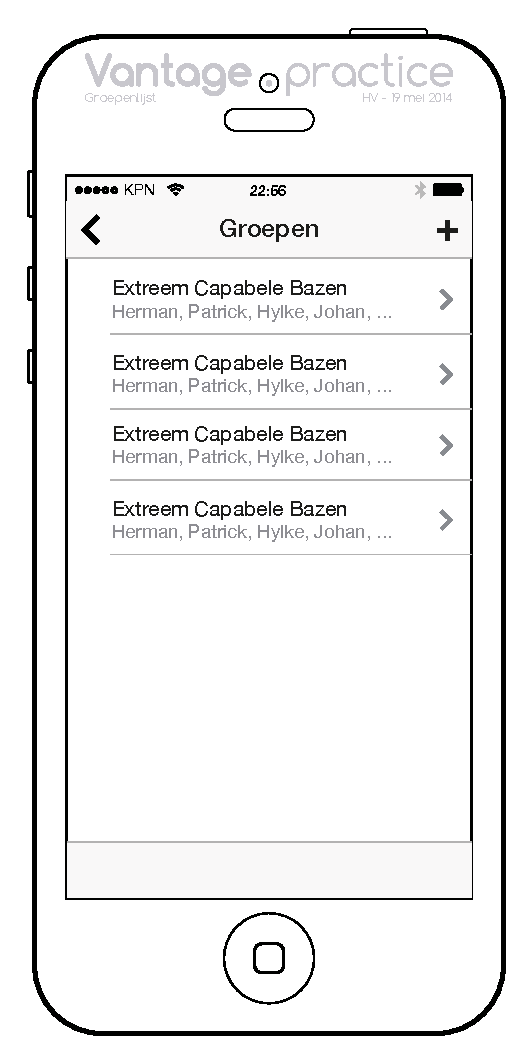
\includegraphics[width=4.5cm]{style/images/designs/12-Groepenlijst}
    \label{fig:groepenoverzicht}
}
\subfigure[Groep Detail]{
    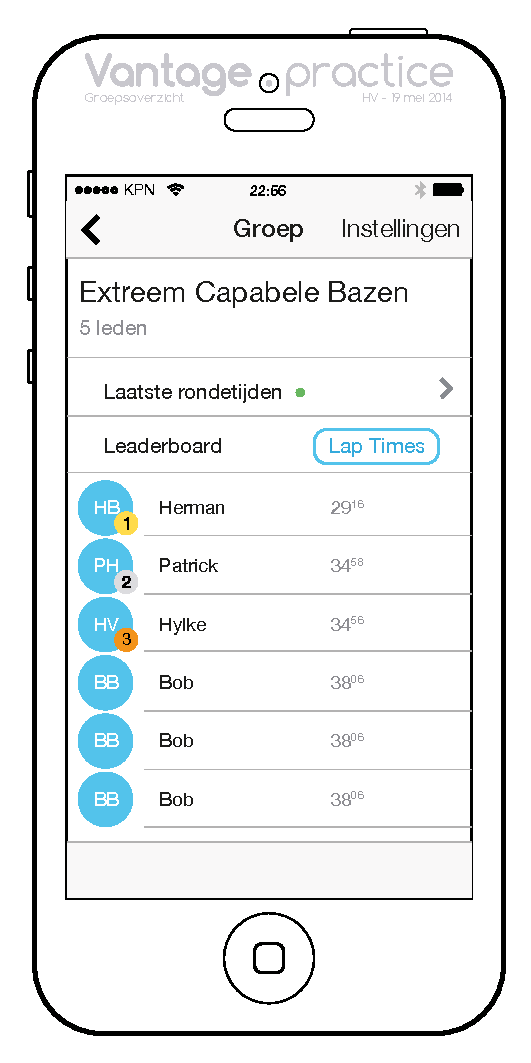
\includegraphics[width=4.5cm]{style/images/designs/13-Groep}
    \label{fig:groep-detail}
}
\subfigure[Groepsinstellingen]{
    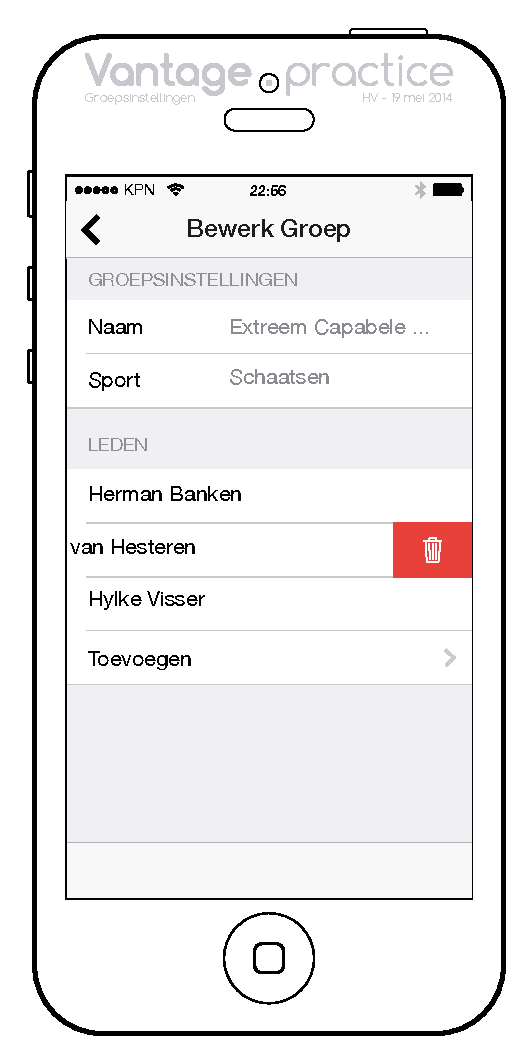
\includegraphics[width=4.5cm]{style/images/designs/14-Groepsinstellingen}
    \label{fig:groepsinstellingen}
}
\caption{Groeps-schermen}
\label{fig:groeps-schermen}
\end{figure}



\chapter{Testresultaten} \label{ch:testplan}
    \label{sec:enquete-resultaten}

Onderstaande tabel bevat de resultaten van de enquête. In totaal zijn er 31 enquête-formulieren ingeleverd. Sommige vragen waren multiple choice en sommige op basis van een schaal naar belangrijkheid, waar 1 onbelangrijk is en 5 erg belangrijk.

\begin{figure}[ht]
  \begin{center}
    \includegraphics[width=\textwidth]{style/images/Enquete1}
  \end{center}
  \label{fig:enquete1}
\end{figure}

\begin{figure}[ht]
  \begin{center}
    \includegraphics[width=\textwidth]{style/images/Enquete2}
  \end{center}
  \label{fig:enquete2}
\end{figure}

\begin{table}[h]
\begin{tabular}{| l | l | l |}
\hline
                         & \multicolumn{2}{l |}{Distributie of}                                                          \\ \hline
                         & Gemiddelde                                     & Standaard deviatie                           \\ \hline
\multicolumn{3}{l}{\textbf{Algemeen}}                                                                                  \\ \hline
Leeftijd                 & 24.1 jaar                                      & 9.0                                          \\ \hline
Geslacht                 & \multicolumn{2}{l|}{70\% man, 30\% vrouw}                                                     \\ \hline
Sporten                  & \multicolumn{2}{l|}{96.7\% Schaatsen, 66.7\% Skeeleren, 6,7\% Baanwielrennen}                 \\ \hline
Sporten overig           & \multicolumn{2}{l|}{Hardlopen, weg-wielrennen, athletiek}                                     \\ \hline
Telefoon                 & \multicolumn{2}{l|}{\begin{tabular}[c]{@{}l@{}}70.0\% Android, 23.3\% iPhone 4+\\ 3.3\% iPhone 2G/3G, 3.3\% Windows Phone\end{tabular}} \\ \hline
\multicolumn{3}{l}{\textbf{Live informatie}}                                                                           \\ \hline
Eigen doorkomsten        & 4.53 uit 5                                     & 0.73                                         \\ \hline
Andermans doorkomsten    & 3.47 uit 5                                     & 1.11                                         \\ \hline
\multicolumn{3}{l}{\textbf{Opgeslagen data}}                                                                           \\ \hline
Inzien doorkomsten       & 4.57 uit 5                                     & 0.63                                         \\ \hline
Inzicht in trainingen    & 4.30 uit 5                                     & 0.84                                         \\ \hline
\multicolumn{3}{l}{\textbf{Sociaal}}                                                                                   \\ \hline
Leaderboards             & 3.23 uit 5                                     & 0.94                                         \\ \hline
Groepen maken            & 3.83 uit 5                                     & 0.91                                         \\ \hline
Suggesties               & 2.73 uit 5                                     & 1.14                                         \\ \hline
Facebook login           & 2.13 uit 5                                     & 1.20                                         \\ \hline
Delen resultaten         & 2.67 uit 5                                     & 1.24                                         \\ \hline
Delen via FB             & 2.00 uit 5                                     & 1.20                                         \\ \hline
Delen via RunKeeper      & 1.63 uit 5                                     & 1.00                                         \\ \hline
\multicolumn{3}{l}{\textbf{Gebruiksgemak}}                                                                             \\ \hline
Audio-cue                & 3.83 uit 5                                     & 1.26                                         \\ \hline
\multicolumn{3}{l}{\textbf{Overig}}                                                                                    \\ \hline
De app willen gebruiken  & \multicolumn{2}{l|}{96.7\% ja, 3.3\% nee}                                                     \\ \hline
Wat de app mag kosten    & € 1.72                                         & 2.13                                         \\ \hline               
\end{tabular}
\end{table}

\newpage

\section*{Verdere functionaliteit opgegeven door respondenten}
\begin{itemize}
\item Tijdsverschillen tussen de rondjes (mobiel bij trainer en rondetijden gelijk terugkijken na oefening)
\item Actuele snelheid zou wel vet zijn. Of een verwachte rondetijd op basis van de huidige snelheid.
\item Trainingen en prestaties delen met endomondo
\item Hardslagmeter, calorieën-schatter. Suggesties voor trainingschema's: lange termijn (intensievere trainingsweek of extensievere trainingsweek) en korte termijn (schaats-schema's die te laden zijn en aan de prestatie gekoppeld worden).
\item Gebruiksvriendelijk, snelheid bv: snel opgestart, etc. De Hockey-WK-app is bijvoorbeeld erg traag en dat is echt niet fijn.
\item Vooraf ingesteld trainingsschema (wat nu gaan doen?) \item Tussentijdse feedback op rijden (tijdens het rijden een piep voor elke "100" meter (niet echt honderd meter, maar herkenbare punten: ingaan bocht/rechte eind, passeren van 1000m start, enz als je een bepaald tempo moet rijden bijvoorbeeld.
\item Tijdens training liever niet vergelijken met anderem, achteraf wel leuk.
\item Misschien een mogelijkheid om je trainingsschema vooraf in te vullen. Dan kun je vervolgens live zien of je dat ook aan het bewerkstelligen bent of dat je niet doet wat je moest doen. Chearleaders die je aanmoedigen als je een beetje achterop raakt op je schema en het boze hoofd van John de Wolf als je gefaald hebt zijn bonus.
\item Metingen op basis van gps en niet alleen via transponders (als dat mogelijk is, vooral handig voor skeeleren).
\item Misschien een rondeteller (zoals die oude mannetjes altijd hebben) voor als je veel rondjes gaat rijden en het zou ook wel vet zijn als je ook je hartslag erbij kan zien, maar dat is voor de echte pro's!
\end{itemize}

\section*{Overige opmerkingen door respondenten}

\begin{itemize}
\item Leuk bedacht, alleen jammer dat je er een transponder voor nodig hebt, wordt het gelijk wel duur. Zou dit ook met GPS kunnen?
\item Het zou wel geniaal zijn als je via je oortjes je hele trainingsschema te horen krijgt en deze vervolgens rijdt en dat de app weet hoe ver je steeds bent. En het lijkt me een vooruitgang dat je real-time weet hoe je snel je de afstanden aflegt, zodat je bijvoorbeeld een vlak of oplopend schema kan rijden.
\item Altijd met telefoon in de hand wordt de ijsbaan niet veiliger van. Denk goed na wanneer je je tel wel/niet in de hand hebt.
\item Een van de belangrijkste punten is wat mij betreft de audiofeedback tijdens het sporten. Het terugkijken van gereden tijden is leuk, maar direct feedback tijdens het sporten werkt voor mij (uit ervaring met RunTastic apps voor hardlopen en wielrennen) erg motiverend.
\item iPhone 4 en verder zijn in dit onderzoek onder een noemer gebracht. Ik merk nu al dat de RunTastic apps, die inmiddels geoptimaliseerd zijn voor iPhone 5C/S, behoorlijk trager werken op iPhone 4. Het zou geweldig zijn als deze app ook soepel runt op iPhone 4. 
\item Werkt de app ook zonder transponder, bijvoorbeeld op GPS?
\end{itemize}

\chapter{Aggregatie Flow} \label{ch:aggregation-flow}

\begin{figure}[ht]
  \begin{center}
    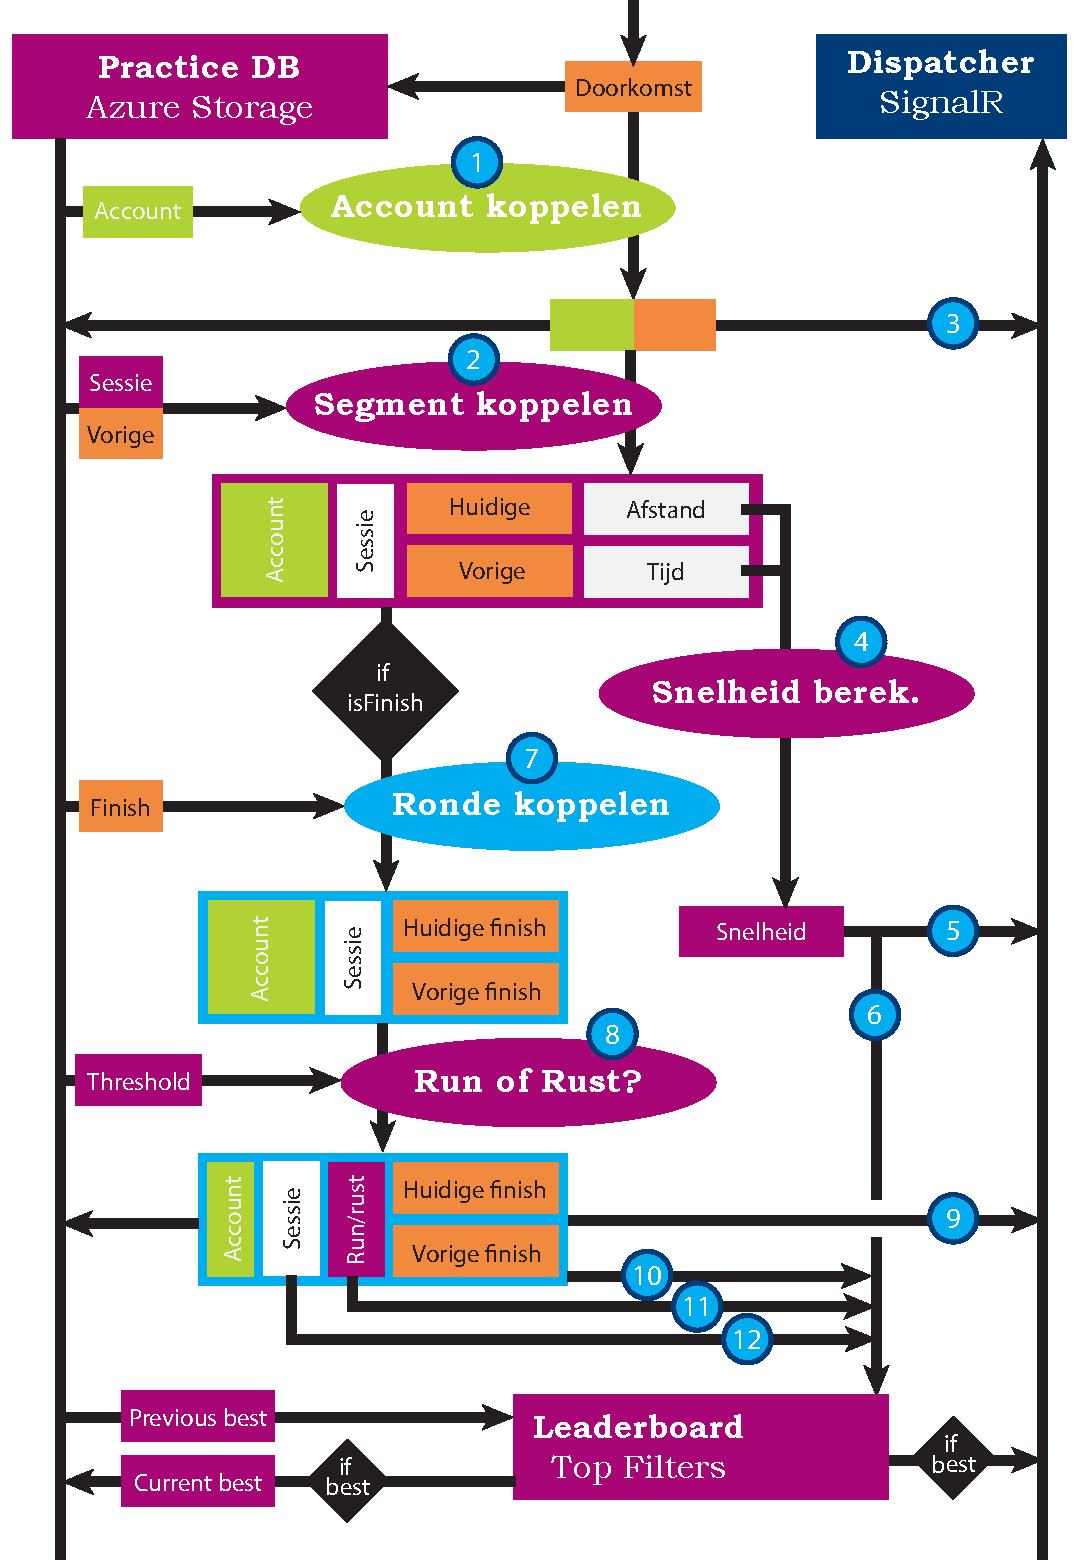
\includegraphics[width=\textwidth]{style/images/Aggregatie-flow}
  \end{center}
  \caption{Flow-diagram van het aggregatie proces}
  \label{fig:aggregatie-flow-large}
\end{figure}

\bibliography{references}

\end{document}